\documentclass[11pt,letterpaper ,oneside ]{book}
\usepackage{graphicx, color}
\usepackage{geometry}
\usepackage{url}
\usepackage{subfig}
\usepackage{amsthm}
\newtheorem{definition}{Definition}
\newcommand{\red}[1]{{\color{red}{#1}}}
\usepackage[]{algorithm2e}

\begin{document}
	
	\begin{titlepage}
		
		\newcommand{\HRule}{\rule{\linewidth}{0.5mm}} % Defines a new command for the horizontal lines, change thickness here
		\center % Center everything on the page
		
		%----------------------------------------------------------------------------------------
		%    HEADING SECTIONS
		%----------------------------------------------------------------------------------------
		
		%\includegraphics[width=\linewidth]{uvaENG}\\[2.5cm]
		\textsc{\Large MSc Artificial Intelligence}\\[0.2cm]
		\textsc{\Large Master Thesis}\\[0.5cm] 
		
		%----------------------------------------------------------------------------------------
		%    TITLE SECTION
		%----------------------------------------------------------------------------------------
		
		\HRule \\[0.4cm]
		{ \huge \bfseries \red{Designing custom inconsistent knowledge graphs}}\\[0.4cm] % Title of your document
		\HRule \\[0.5cm]
		
		%----------------------------------------------------------------------------------------
		%    AUTHOR SECTION
		%----------------------------------------------------------------------------------------
		
		by\\[0.2cm]
		\textsc{\Large \red{Thomas de Groot}}\\[0.2cm] %your name
		\red{11320303}\\[1cm]
		
		
		%----------------------------------------------------------------------------------------
		%    DATE SECTION
		%----------------------------------------------------------------------------------------
		
		{\Large \today}\\[1cm] % Date, change the \today to a set date if you want to be precise
		
		\red{36 EC}\\ %
		\red{September 2018 - March 2019}\\[1cm]%
		
		%----------------------------------------------------------------------------------------
		%    COMMITTEE SECTION
		%----------------------------------------------------------------------------------------
		\begin{minipage}[t]{0.4\textwidth}
			\begin{flushleft} \large
				\emph{Supervisor:} \\
				\red{Dr \textsc{Stefan Schlobach } }% Supervisor's Name
			\end{flushleft}
		\end{minipage}
		~
		\begin{minipage}[t]{0.4\textwidth}
			\begin{flushright} \large
				\emph{Assessor:} \\
				\red{Dr  \textsc{Joe Raad}}\\
			\end{flushright}
		\end{minipage}\\[2cm]
		
		%----------------------------------------------------------------------------------------
		%    LOGO SECTION
		%----------------------------------------------------------------------------------------
		
		\framebox{\rule{0pt}{2.5cm}\rule{2.5cm}{0pt}}\\[0.5cm]
		%\includegraphics[width=2.5cm]{figure}\\ % Include a department/university logo - this will require the graphicx package
		\textsc{\large \red{institute name}}\\[1.0cm] % 
		
		%----------------------------------------------------------------------------------------
		
		\vfill % Fill the rest of the page with whitespace
		
	\end{titlepage}
	\pagenumbering{roman}
	
	
	\newpage
	\chapter*{Abstract}
	Based on formal semantics, most of the knowledge graphs on the Web of Data can be put to practical use. Unfortunately, a significant number of those graphs are logically inconsistent. This makes reasoning impossible and the knowledge formally useless. While methods exist to deal with contradictions, no systematic way exists to evaluate these algorithms on large realistic knowledge graphs. Even worse, there is not even a methodology for analysing inconsistency in graphs in the first place. \\
	
	While large inconsistent knowledge graphs are available, their size often prohibits their usage for benchmarking. Thus, current research often resorts to synthesised knowledge graphs. In this paper, we present a formal notion of `anti-patterns'; generalised basic graph patterns that describe contradictions in knowledge graphs. We present an extraction pipeline that retrieves explanations for contradictions in the LOD-a-lot collection of knowledge graphs and generalise them into what we call `anti-patterns'. We enlist an (almost) complete set of `anti-patterns' found in the LOD-a-lot. Next, we evaluate the set `anti-patterns` on their intrinsic characteristics. Finally, we introduce two usages of those `anti-patterns': first, for knowledge graph analysis, and secondly, for generating systematic samples from knowledge graphs. We showcase the two implementations by analysing a set of knowledge graphs and from these we generate configurable inconsistent subontologies of variable size. 
	
	\newpage
	\tableofcontents
	\newpage
	\pagenumbering{arabic}
	
	\chapter{Introduction}\label{Introduction}
	\section{Motivation}
	\textit{Background}. Blaise Pascal once said, "A contradiction is not a sign of falsity, nor the lack of a contradiction a sign of truth." Large amounts of data have been made available for everyone. Multi-billion facts – also called statements, or tiples – are now the standard for a linked-data dataset instead of the exception. Due to that, we are sitting on a large amount of open data. The problem is that we do not know if all the facts in the dataset can be considered the truth. We know that data is inherently dirty. It is also known that finding new facts from the data is impossible if the data holds facts that are contradictory. While there is active development in solving the problem of contradictions in datasets. For example, ignoring the parts that hold contradictory statements and still use the rest of the dataset. Only this method would still miss facts that could have been found if we removed only the contradictory facts and used a dataset that is devoid of contradictions. So while a contradiction is no sign of a false dataset, a lack of contradictions would certainly be a step in the right direction to the truth.\\
	
	\textit{Motivation}. Finding and removing contradictions from datasets in a simple and systematic way has a number of benefits. Firstly we could study the types of mistakes that have been made in the datasets. How these mistakes are made, by automatic algorithms, or by people in the process. This helps to find problems at the source, the generation of the data, instead of later in the process. \\
	Secondly, we can generalize the contradictions and design blueprints that can be used to describe groups of contradictions, standardized to apply to other datasets as well. Thirdly, we could use the found contradictions to analyze existing datasets. We can use the blueprints to find if there are contradictions found in other datasets. 
	Finally, we can use the found contradictions blueprints, to build benchmarks designed to test tools, that require large datasets with known characteristics.\\
	
	\textit{Method} In this work, we developed a method of extracting contradictions from linked datasets. We call these generalised contradictions `anti-patterns', as these contradictions can be seen as common mistakes made in the dataset. We describe a formal notion of `anti-patterns' in chapter \ref{AntiPatternDefinition}.\\
	
	For the retrieval of the `anti-patterns', we have designed an extraction pipeline that can find any `anti-pattern' for an arbitrary, inconsistent linked dataset. Algorithmic we can prove that we can retrieve the complete set `anti-patterns'. We show this by retrieving such `anti-patterns' from the LOD-a-lot\cite{JavierD:2017} a dataset containing 28 billion facts. We use the set of `anti-patterns' found in the LOD-a-lot as input for the two implementations. The two implementations we designed are analysis for inconsistent knowledge graphs and a sampling method. Both these implementations make extensive use of the found `anti-patterns'. 
	
	\section{Research questions}
	\textit{Research questions}. The main research goal of this work is to discover an effective method of finding contradictions and generalize the contradictions we found into `anti-patterns'. In the above section, we already described our method informally. To formalise our goals we wrote down the following research questions that form this paper.
	
	\begin{itemize}
		\item \textbf{RQ1}: Can we describe and define a formal definition for general contradiction patterns, where general contradiction patterns are inconsistent subgraphs which are persistent throughout all natural knowledge graphs?
		\item \textbf{RQ2}: How can we retrieve the general contradiction patterns that have occurred in natural knowledge graphs? 
		\item \textbf{RQ3}: What classifications are there which can classify groups of general contradiction patterns? And what main characteristics can describe the classes of contradiction patterns best? Can we use these commonalities to give better qualitative and quantitative information about the graph?
		\item \textbf{RQ4}: Are there methods, or can we design methods that could benefit from using general contradiction patterns in their algorithm? 
		\begin{itemize}
			\item Are we able to improve analytics about contradictions for large linked datasets, by giving qualitative and quantitative information about linked datasets?
			\item Can we use the anti-patterns, to build benchmarks. Benchmarks that have been sampled from large, but inconsistent datasets with general contradiction patterns. Would it be possible to keep the sampled characteristics invariant from sampling?
		\end{itemize}
	\end{itemize}
	
	\section{Contribution}
	\textit{Contributions}. 
	The main contributions in this work, with respect to the research questions, can be described in threefold.
	\begin{itemize}
		\item First, we give a formal definition of `anti-patterns' we use to describe common occurring generalised contradictions that we found in the linked datasets. We use these definitions throughout this work to describe the generalized patterns.
		\item Secondly, we design an extraction pipeline that can extract `anti-patterns' from any arbitrary knowledge graph. We show that this method works by extracting "almost" all contradictions. We made all the `anti-patterns' available to use on the web.
		\item Thirdly we show that `anti-patterns' can be used to analyse inconsistent knowledge graphs and to sample inconsistent knowledge graph systematically.
	\end{itemize}
	
	\textit{Experiments and implementations}. We test our extraction pipeline on two points. Firstly if it is possible to retrieve all `anti-patterns' from a linked dataset. This is done by using a benchmark dataset, the "pizza-ontology". The "pizza-ontology" is a dummy dataset that holds only a small number of facts and a few contradictions, simple enough to check by hand. Secondly, we test our extraction pipeline on the LOD-a-lod, one of the largest open datasets. We use the `anti-patterns' from this dataset as input for analysis and sampling.\\
	
	Finally, we have selected two implementations to evaluate our method with real-world examples. Firstly, we have designed a system that can analyse linked datasets. The system retrieves all the  `anti-patterns' based on contradictions in the LOD-a-lot and calculates the number of times the `anti-patterns' occur in the linked datasets. Then, the system returns a detailed report of characteristics of linked datasets.
	Secondly, we show the implementation that samples a linked dataset that can be tweaked with a user-specified sample-size and the number of contradictions per `anti-patterns'. \\
	
	\textit{Findings}. We have tested our pipeline by extracting an `almost' complete set of `anti-patterns' from the LOD-a-lot\cite{JavierD:2017}, which we made available \\ \url{https://thomasdegroot18.github.io/kbgenerator/Webpages/statisticsOverview.html}. We developed a set of characteristics that can be used to describe `anti-patterns' more concisely. 
	We show that there is a correlation between the size of the `anti-pattern' and the amount of different `anti-patterns'. 
	We tested two implementations by processing a set large knowledge graphs, DBpedia\cite{DBpedia}, and YAGO\cite{YAGO}, DBLP\cite{DBLP}.
	We found that the `anti-patterns' give us a more detailed explanation about the contradictions in the inconsistent knowledge graph. 
	We show how the characteristics change between the dataset. We show that the sampled knowledge graphs match the set characteristics given by the user, and also match the characteristics of the original knowledge graph.\\

\section{Outline}
In chapter \ref{Background} the different concepts used in this work are introduced. Chapter \ref{RelatedWork} explains the related work, which has been done by others on which this work is based.
In Chapter \ref{Method} we explain more in detail how the method of `anti-pattern' retrieval works. Chapter \ref{internalvalidation} explains the experiments we performed to validate the internal proceedings of the algorithm. Chapter \ref{Implementation} showcases the possible applications that make extensive use from the `anti-pattern' that we retrieved in the method. In Chapter \ref{externalvalidation} we show how the applications perform, we set in the introduction, and analyse the results. We conclude with a conclusion, with an extension of future work in chapter \ref{Conclusion}.
	
	
	\newpage
	\chapter{Background}\label{Background}
	In this chapter, we introduce the set of essential preliminary concepts that are needed to understand the research that we present in this work. To help the reader, we also introduce a set of examples that are used in this paper to help the reader understand.
	
	\section{Knowledge graph}\label{graphElements}
	Knowledge graphs are the basis of some of the most advanced systems, Google, for example, uses a knowledge graph to enhance its search results, with information about the search question shown in the box next to the question. Searching for "Tim Berners-Lee", not only shows the results but also shows relevant information about him. The information that is shown comes from the knowledge graph Google has built. But what is exactly a knowledge graph?
	
	\textit{Knowledge graph}. 
	A knowledge graph can be seen as a part of a knowledge-based system. Where the knowledge graph stores all the statements, which represent the facts about the known world. The second part of the knowledge-based systems is the reasoner, which will be discussed in a later part of this chapter. A knowledge graph consists of a large amount of RDF triples, also known as statements or facts.
	
	we derived a formal notion of a knowledge graph from Paulheim et al. \cite{HeikoP:2016}:
	\begin{definition} 
		“A knowledge graph (i) mainly describes real-world entities, and their interrelations, organized in a graph, (ii) defines possible classes, and relations of entities in a schema, (iii) allows for potentially interrelating arbitrary entities with each other and (iv) covers various topical domains.”
	\end{definition}
	
	\textit{RDF triple}. These facts can be anything. For example, Lisa owns Sam, or Sam a is of type Rabbit, Sam is Brown. Each RDF triple consists out three elements.
	The three elements are $<$Subject$>$, $<$Predicate$>$, and $<$Object$>$. Where the subject and the object are two entities and the predicate is the link between them, describing the relation between the two entities. 
	
	There are a few problems with writing $<$Lisa$>$ $<$owns$>$ $<$Sam$>$. What if there is more than one Sam? To counter this, we use (Uniform Resource Identifier) or otherwise known as URI to define an entity. A URI is a set of characters that unambiguously identifies an abstract or physical resource. Lisa would become \\$<$https://data.persons.com/world/Europe/Netherlands/122341$>$ $<$https://names.org/hasname$>$ "Lisa". Where this statement links the identifier, to the name Lisa. Now every time Lisa is mentioned the identifier is used. 
	The second problem that needs solving is the standardization of the relation description, such that each relation type has a unique meaning, which can be related back to a language describing this meaning. This creates the possibility to start reasoning. Because if we know the meaning of the fact we can learn new facts. Before we can get to reasoning, we need to have a language defined to reason with. The most common reasoning languages are RDF, RDFs, and OWL.
	
	\textit{RDF} \cite{rdfPrimer:2014} stands for \textbf{r}esource \textbf{d}escription \textbf{f}ramework and is a method of storing data in triple format. These statements, consisting out of the $<$Subject$>$, $<$Predicate$>$, $<$Object$>$ can hold different types. The subject can be defined as a URI or a blank node. The predicate represents the relation between the Subject and the Object and is always defined as a URI. Finally, the object is the second resource. This can be a URI, blank node or a literal.
	RDF is designed to exchange information between processes and applications without the intervention of humans. The goal was to build a framework that is designed link resources without having to add expensive parsers to convert the information to the correct format every time a new process is added which wants to use the information.\\

\textit{RDFS} \cite{RDFSchema:2014} is the extension of the RDF language with an RDF schema. With this we can extend the knowledge created by RDF and add for example labels to certain concepts and give more structure to the data. With RDFs we can define Classes, resources and literals as well as ranges and domains for predicates. Giving the ontology a more rich description. With this information it is finally possible to do extensive reasoning. Thus making it possible to infer new facts from the knowledge of other triples.\\

\textit{OWL}\cite{OWLPrimer:2012}, the Web Ontology Language, designed to represent the language that can describe things and set of things well with regards to relations. OWL can also be seen as an extension to RDF, and is used in combination with RDF(s). With OWL we define more implicit relations such as an subClassOf relation. For example a definition of subClassOf(Mammal, Vertibrae) and subClassOf(Rabbit, Mammal). This makes it possible to reason that subClassOf(Rabbit, Vertibrae) is also a type of relation that exists. 

	\textit{Basic Triple Pattern}. The problem with RDF triples is that each triple is instantiated, meaning that all triples have a value, which can be a URI, or a literal,  a fixed value in the statements. 
	To have the ability to generalise within a knowledge graph, we use Basic triple patterns(BTP). BTPs can be seen as RDF triples, but where it is possible to change one, two or all three elements from the RDF triple into variables. With an uninstantiated BTP, we can use SPARQL to ask a question to the knowledge graph and retrieve instantiated BTPs back. Alternatively, we can check with an instantiated BTP if it exists in the knowledge graph.\\
	
	\textit{Basic Graph Pattern}. A basic graph pattern (BGP) is a set of basic triple patterns and forms the basis of query matching. The basic graph pattern
	can consist of BTPs that are connected.
	Alternatively, the BGP consists out of disconnected BTPs. Same as the BTP a BGP can be instantiated, without variables, or uninstantiated, thus parts of the BGP have been replaced with variables. With basic graph patterns, we can ask more informed questions to the knowledge graph, or find if an instantiated BGP exists in the knowledge graph.\\
	
	\textit{Ontology} An ontology is a description of a collection of concepts, most of the time, the ontology is focussed on a specific domain, such as for example biology, auto races, or political parties. With an ontology, we can describe concepts with the use of several components. The components consist of:
	- Individuals: instances of objects, which can be seen as instantiated or grounded elements of classes. This can be for example the person "Tim Berners-Lee", "Lisa", and "Sam".
	- Classes: groups of individuals can be classified within a class. "Persons" or "Rabbits"
	- Both classes and individuals can have attributes, also called properties or features. A person has a height, or a weight has a language he or she can talk. Different classes can have different properties. 
	- Relations are connections between individuals, and classes, describing links between individuals. A person can know another person. "Lisa" is of type person. 
	
	An ontology can be seen as a set of triples, with each of the triples a combination of the above, describing the elements of the ontology.
	
	\section{Reasoner}
	Reasoning is the method in which we use logic and facts to reason to a conclusion. In knowledge graphs we use reasoning to derive new facts from the knowledge graph, facts that were not explicitly written down. Reasoning is also used to verify facts that already exist in the knowledge graph. This could mean that facts are contradictory to each other resulting into an contradiction.
	
	
	\subsection{Reasoning types}
	Reasoning is deriving facts from the ontology or knowledge base that has not yet been explicitly denoted. We can classify reasoning in several different subcategories, that are not a lot different from each other but can have other optimized algorithms specialized in solving the different subcategories.
	\begin{itemize}
		\item Satisfiability of a concept, determining if a description of a class or concept is not contradictory. As we have shown in the examples, the goal of this reasoning type is if  we can find an individual that satisfies the Class without creating a contradiction in the knowledge graph. 
		\item Subsumption of concepts, can we determine if a Class C is more general than Class D
		\item Consistency with respect to the ontology. The goal is to check if the concepts we defined in the ontology match with the actual usage of the ontology. Meaning that we want to determine whether individuals do not violate descriptions and statements that are described by the ontology.
		\item Check an individual - check whether the individual is an instance of a class
	\end{itemize}
	In this work, we will focus on satisfiability, but instead of finding the concepts that are satisfiable we will instead look for the opposite, and find the concepts and individuals that are unsatisfiable — thus finding if the knowledge graph is inconsistent. Which means that the graph is holding contradictory statements. So what makes a graph inconsistent?
	
	\textit{Inconsistency} An inconsistent knowledge graph is a graph that has one or more statements that are inconsistent with each other. A knowledge graph can have several types of inconsistency. It can be grammatically inconsistent. This happens when a statement is defined with the incorrect datatype, a grammatical error of sorts. Here we focus on semantical inconsistency. This occurs when constraints that have been set by the language used in the knowledge graph have been broken. Shown in example \ref{fig:Example1}. This can happen when an instance is linked to two classes that are disjoint with each other. To find where a knowledge graph is inconsistent we use justifications.   
	
	\textit{Justification}. A justification\cite{Horridge:2009} is a set of axioms that acts as an explanation for an entailment.
	Formally, a justification is a minimal subset of the original axioms which are sufficient to prove the entailed formula. In this paper, we interpret a justification as an explanation of contradiction. Given that our knowledge graphs are sets of triples, our justifications are instantiated BPGs and are always a minimal set of axioms for a single contradiction. \\
	
\begin{definition} 
	Let $G$ be an knowledge graph such that $G \models \eta$. $J$ is a justification for $\eta$ in $G$ if $J \subseteq G$, and $J \models \eta$, and for all $J'\subseteq J, J' \not\models \eta$.  \cite{Horridge:2009}
\end{definition}
	
	\section{Example introduction}
	Now that the basic notions of a knowledge graph are explained we will show a knowledge graph work in two examples. 
	\begin{figure}
		\centering
		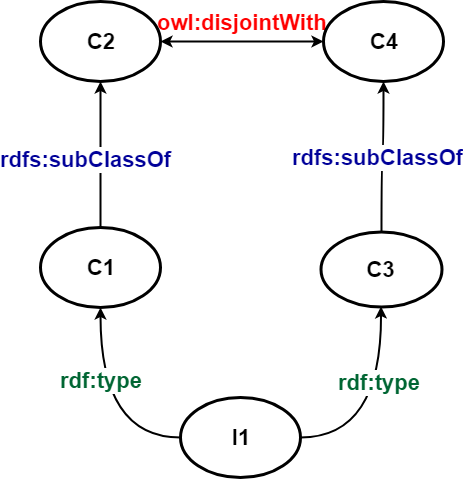
\includegraphics[width=\linewidth]{images/Example1.png}
		\caption{Example contradiction 1.}
		\label{fig:Example1}
	\end{figure}
	\begin{figure}
		\centering
		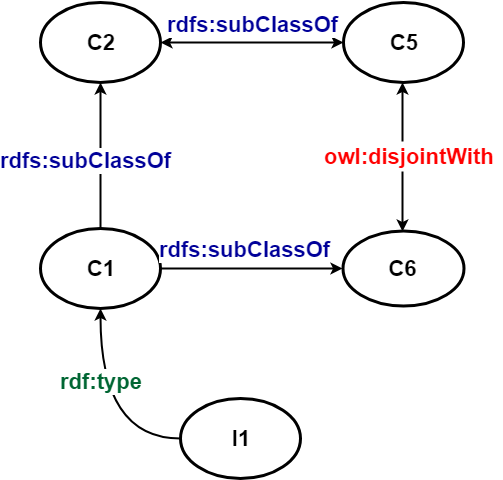
\includegraphics[width=\linewidth]{images/Example2.png}
		\caption{Example contradiction 2.}
		\label{fig:Example2}
	\end{figure}
	
	\textit{Example 1}. The first image\ref{fig:Example1} shows a simple contradiction, in this example we see an individual[I1], that is of two classes, for example "Monaco" is of type \textit{city in Europe}[C1] and of type \textit{country in Europe}[C3]. This is still correct; an instance can be of two different types. Now we define that a \textit{city in Europe} is a subclass of a \textit{City} and that a \textit{country in Europe} is a subclass of a \textit{Country}. This is still a correct assumption. We now define that a \textit{City} cannot be a \textit{Country} or the other way around by saying that both classes can never have an individual in common. We now created a contradiction, as \textit{Monaco} is an individual of both, but it can not be.\\
	
	Fixing this contradiction is possible, but it means that we need to change some things, we can either remove the disjoint axiom, meaning that now we can have a \textit{City} that is also a \textit{Country}. We could also split \textit{Monaco} into \textit{Monaco(City)} and \textit{Monaco(Country)}, which is also a possible solution. Both solutions have their advantages and disadvantages.\\
	
	\textit{Example 2}. The second example\ref{fig:Example2}, shows a different type of contradiction. This time we only have one rdf:type relation. This individual belongs to only one class, For example we have a individual \textit{Lisa}[I1] now is of the class \textit{Person}[C1], This class has two subClass relations, with \textit{RationalBeing}[C6] and \textit{Mammal}[C2]. Where \textit{mammal}[C2] is also a sub class relation with \textit{ImpulsiveBeing}[C5]. Which in turn is disjoint with \textit{RationalBeing}[C6]. This makes the circle complete and generates another contradiction, as both \textit{ImpulsiveBeing}[C5] and \textit{RationalBeing}[C6] have an individual[I1] in common. \\
	
	
	\chapter{Related Work}\label{RelatedWork}
	This section is an review of the work done by other on which we built our work. More specifically, we show the previous work done for our designed method, the analysis application and the sampling application. 
	
	\section{Method}
	Making a knowledge graph consistent has been an old problem, and solutions have been proposed as early as 1956 by Toulmin in his book \cite{toulmin:1956}, in which the solution is proposed by revising the base, choosing to reason only over the consistent subbases, expanded upon by Gabbay et al\cite{Gabbay:1994}. The second solution is to change the inference of the reasoner to fit the inconsistency and can be seen as the first approaches to paraconsistent reasoning, such as done by Kaminski et al.\cite{Kaminski:2015}.
	
	With reasoning used in most software algorithms, the research done analysing inconsistent knowledge graphs has only been emerging in the last decade with the introduction of justifications by Horridge et al.\cite{Horridge:2009}. In their paper, the writers describe the framework used to retrieve the justifications from inconsistent knowledge graphs as minimal subsets of the graphs preserving the inconsistency. This forms an integral part of our algorithm. In the paper, they also explain why it is often time-consuming to retrieve all justifications for ontologies. In the paper by T\"{o}pper et al.\cite{Topper:2012} they, propose a solution to identify contradictions in DBpedia, for a single type of contradiction. With the extraction of our `anti-patterns', we have a generalised approach that works for any contradiction on any knowledge graph. \\
	
	Previous work locating contradictions has been done by Eiter et al.\cite{Eiter:2010}, in their work, they propose two methods to locate contradictions created by combining knowledge graphs. The contradictions they focus on are contradictions that span separate knowledge graphs. They specifically focus on the bridge rules, rules that connect knowledge graphs, which can bring contradictions to light. Their method forms the basis for McAreavey et al.\cite{McAreavey:2014}. In the work for McAreavey, they introduce the MINUS algorithm for finding contradictions in the knowledge graph, in their work they look for groups of minimal inconsistency sets. The method is further improved by Zhi et al.\cite{Zhi:2015}. In their work, they have implemented an improved algorithm which uses subsets to locate inconsistencies in the knowledge graphs. In their papers, however, their goal is finding these sets for a specific knowledge graph, where in our case we generalize the inconsistencies to be used in all knowledge graph. The second design decision is that they are staying in first-order logic while we are also making the step to description logics.
	
	All three methods look for inconsistency in their respective knowledge bases. The problem with all three techniques is that they are designed from a theoretic viewpoint. All three work with solving the inconsistency problem for all cases. This makes the algorithms complex, and all have problems with solving it for larger knowledge graphs. If we look at our method, we can see that ours also solves the inconsistency problem for all arbitrary knowledge graphs. But we also have an algorithm that finds almost all contradictions for any inconsistent knowledge graph quicker With the `anti-patterns' we cover most contradictions in the data such that finding contradictions is also possible by SPARQL queries alone.
	
	Our method reuses part of the method that has been developed by Azad Noori et al\cite{Noori:2015}. In this paper, they propose an efficient algorithm for pathfinding that we use in our subgraph generation and in our sampling.
	
	\section{Analysis}
	Paulheim \cite{HeikoP:2016} showcases the need for a standardised evaluation method. In the survey, they show that researchers sometimes choose different knowledge graph(s) according to their needs, this makes it harder to compare different algorithms. Removing this discrepancy would benefit all of us.
	
	F\"arber et al. \cite{MichaelF:2017} give an in-depth comparison of several large knowledge graphs, and demonstrates that knowledge graphs have different characteristics. The paper by F\"arber et al. \cite{MichaelF:2017} is expanded upon by Debattista et al. in \cite{Debattista:2018}, in which they analysed 130 datasets from the Linked Open Data Cloud using 27 Linked Data quality metrics. Both papers show that each graph has a different underlying structure and in theory, this even can result in different behaviour of algorithms.
	
	The paper by Peter Bloem and Steven de Rooij\cite{BloemP:2018} is a good use-case in which we could implement our anti-patterns for analysis. With a combination of implementations, we could make statistical inferences about whether or not `anti-patterns' occur with regularity. Which would incredibly useful for making automatic software.
	
	\section{Sampling}
	In the paper by Jure Leskovec and Christos Faloutsos \cite{Leskovec:2006} several sampling techniques are proposed and compared, and with it they show that even naive sampling such as random walks and 'forest fire' show accurate results, even sampling to 15\% of the original size. 
	Albatross sampling by Jin et al.\cite{Jin:2011}, shows a sampling technique designed for loosely connected or disconnected networks, especially for social networks, while this technique is useful for sampling graph networks, as the algorithm will give an even more accurate sample, but due to an extra constraint implemented in our sampling method, this sampling technique could not be applied.
	
	In the paper by Kurant et al.\cite{Kurant:2011}, they explain the bias that forms when implementing breath first sampling.
	While this paper has no direct effect on the implementation, the information described in the paper is useful to explain why our samples have some discrepancies when it comes to the differences in indegree and outdegree. 
	
	Finally Rietveld et al.\cite{Rietveld:2014} shows that sampling for targeted use, in their case SPARQL coverage is possible, this shows that sampling a knowledge base, for targeted cases can generally be relevant for a multitude of reasons.
	
	
	\newpage
	\chapter{Approach}\label{ProblemDefintion}
	In this chapter, we introduce a formal approach to the problem. The problem formalization is crucial in the aim of this work in order to understand the method we propose in the next section.
	
	\section{Problem Description}
	Most large knowledge graphs have contradictions, but with reasoners only being able to reason on smaller knowledge graphs, we do not know much about the composition of the contradictions in the knowledge graphs. Understanding how the contradictions have formed, or where the contradictions occur, is crucial information when we want to develop better tools that can handle larger knowledge graphs. The second problem is that, while implementing solutions on a large scale is preferable, testing and benchmarking on smaller knowledge graphs that match existing knowledge graphs is preferable to dummy knowledge graphs. A natural knowledge graph that has known properties and contradictions instead of synthesised knowledge graphs is always preferable. 
	
	To grasp the issue at hand, we split the problem into three parts. The first part is to locate the contradictions within the knowledge graph. Only contradictions that are known can be treated as such. Sampling later in the pipeline would only work with contradictions that are known beforehand to sample accordingly.
	The second part of the problem is the knowledge graph analysis. Analysing the graph gives useful statistics about the knowledge graph, and helps us understand the knowledge graph also with respect to the found contradictions in the first part.
	
	The final part of the problem is the sampling of the knowledge graph. Is it even possible to sample from the original knowledge graph and keep the characteristics? Moreover, can we make sure that the sampled graph still holds the number of inconsistencies we want the graph to have? 
	
	\subsection{Research questions}
	To formalize the problem description, the following research questions are formulated.
	\begin{itemize}
		\item \textbf{RQ1}: Can we describe and define a formal definition for general contradiction patterns, where general contradiction patterns are inconsistent subgraphs which are persistent throughout all natural knowledge graphs?
		\item \textbf{RQ2}: How can we retrieve the general contradiction patterns that have occurred in natural knowledge graphs? 
		\item \textbf{RQ3}: What classifications are there which can classify groups of general contradiction patterns? And what main characteristics can describe the classes of contradiction patterns best? Can we use these commonalities to give better qualitative and quantitative information about the graph?
		\item \textbf{RQ4}: Are there methods, or can we design methods that could benefit from using general contradiction patterns in their algorithm? 
		\begin{itemize}
			\item Are we able to improve analytics about contradictions for large linked datasets, by giving qualitative and quantitative information about linked datasets?
			\item Can we use the anti-patterns, to build benchmarks. Benchmarks that have been sampled from large, but inconsistent datasets with general contradiction patterns. Would it be possible to keep the sampled characteristics invariant from sampling?
		\end{itemize}
	\end{itemize}
	
	\section{Method}
	The first step that we need to take is to define an `anti-pattern' and retrieve the `anti-patterns' from knowledge graphs. The method we developed is not based on any work that has been previously created. Instead, we opted to develop our own method. The method is designed specifically to retrieve `anti-patterns' from large knowledge graphs. Which are generalised contradictions, and can be seen as common mistakes made in a dataset. We described a formal notion of `anti-patterns' in chapter \ref{AntiPatternDefinition}. Our method for retrieval is a three-stage pipeline. The results of the previous stage flow into the next stage. The input is a natural knowledge graph; in our case, this is the LOD-a-lot\cite{JavierD:2017} a dataset containing 28 billion statements. The output from the final stage will be the found `anti-patterns'. 
	
	\subsection{Proposed Applications}
	With the `Anti-patterns' found, we propose two implementations that benefit greatly from `anti-patterns', The first being analysis for inconsistent knowledge graphs and the second a sampling method which uses `anti-pattern' in its sampling. The first implementation, analysis takes any arbitrary knowledge graph, and analyses this graph on the basis on a number of characteristics including the found `anti-patterns'. Which helps us understand what types of `anti-patterns' occur in a knowledge graph, giving us a better overview of inconsistent knowledge graphs in general, answering our second research question.
	
	The second implementation, sampling is a common use case for other research topics as well. The reason for this implementation is that benchmarking for a number of research topics, which use knowledge graphs that have been specifically designed for testing, such as Lehigh University Benchmark, which is an ontology data generation tool. While this could work for testing, it could also be that algorithms perform not as well on natural knowledge graphs. But due to the size of natural knowledge graphs, such as YAGO, DBpedia, and LOD-a-lot, it will be time-consuming to test on these knowledge graphs without knowing if the algorithm even works. To combat this sampling can be used to retrieve a smaller part of the knowledge graph we want to test on and use this sample to test the algorithm on. While sampling is a good practice to shrink the test space, it could be that the sampling loses some of the characteristics of the original knowledge graph. 
	
	We designed a different sampling technique that uses `anti-patterns' as a basis for sampling. This sampling technique uses the found `anti-patterns' to build a knowledge graph that is inconsistent, with respect to the original knowledge graph. Secondly, the sampling can be used to sample a knowledge graph with only a specific set of `anti-patterns'.
	
	\subsection{Proposed Experiments}
	Now that we set up our method, we show how this method performs with different experiments. 
	Firstly we test if we can retrieve `all' justifications from the knowledge graph, due to the extraction process in the final algorithm we can not guarantee that we can extract every contradiction from the knowledge graph. Which means that it is possible for the method to miss contradictions, and thus it can be possible that we miss the accompanying `anti-patterns' that we could have derived from the contradictions. To test the hypothesis that we still can retrieve most to all `anti-patterns' we developed an experiment by extracting all the contradictions from the pizza-ontology. We choose this ontology as it is a small ontology with concrete statements that can be easily understood. It makes it possible to check by hand if the amount of `anti-patterns we found, matches the amount of `anti-patterns' we found with our extraction method.
%	REWRITE INSERT EXPERIMENT DESCRIPTION:
	
	We test if we can analyze knowledge graphs, we have two inconsistent knowledge graphs, DBpedia, DBLP and YAGO, both with known contradictions. We retrieve the statistics about the knowledge graph. We then retrieve all the `anti-patterns' that have instantiated contradictions in the knowledge graph. 
	With this experiment, we want to show the use of `anti-patterns' to get a better understanding of how inconsistent knowledge graphs are formed, and what types of `anti-patterns' are more common than others.
	
	Finally, we test if we can sample from an inconsistent knowledge graph. We examine this by experimenting with a set of large knowledge graphs and test if we have replicated the original knowledge graph in a smaller variant.
	
	\newpage
	\chapter{Defining and Finding `Anti-patterns'}\label{Method}
	\section{Anti-pattern definition}\label{AntiPatternDefinition}
	In this section we will introduce the term `anti-pattern'. We will come to a definition of what a `anti-pattern' exactly is, and how we can derive `anti-patterns' from sets contradictions. \\
	
	As explained in chapter \ref{graphElements}, a justification is a description of a single contradiction. We can see it as proof that an ontology is inconsistent. Each justification is an instantiated BGP, within the knowledge graph. Due to the instantiation, the justification can only describe one contradiction and is thus limited to a single knowledge graph. To use justifications in other knowledge graphs, for instance, to check if this knowledge graph has the same contradiction, without having the same statements, we need to generalize the justification.
	
	If for example, we have a knowledge graph describing the contradictions in the knowledge graph of Countries in Europe, wherein we wrongfully declared Monaco a city and a country, without the consideration that they are disjoint(see example \ref{fig:Example1}). Now we need to quickly check if this contradiction happens in the knowledge graph for Countries in Asia as well. If we do not know how to generalise the contradiction to an `Anti-pattern' we either have to check the relations for all elements in the graph to check if they can match the pattern, or we need to use a reasoner to find the same mistake again only now in the knowledge graph for Asian Countries.\\
	
	For generalization we created `anti-patterns'. `Anti-patterns' are generalisations over justifications. To transform a justification into an `anti-pattern', we remove all information on the subject and object position of the BGP. Removing the information on the predicate position("owl:disjointWith", "rdfs:subclassOf", "rdf:type", etc) would break the contradiction, as if it would be possible to match a "rdfs:subClassOf" on the place where the "owl:disjointWith" belongs. This would make the contradiction no longer a contradiction. Except for the cases such as a predicate defined with "rdf:range" and "rdf:domain" where we do sometimes need to replace the predicate with a variable. 
	Now that we removed all the information that blocks generalization, we are left with the `anti-pattern'. Now the `anti-pattern' can be used to match various inconsistent justifications in the knowledge graph. We define an \textit{`Anti-pattern'} in the following definition:\\
	
	\begin{definition} 
		An \textit{`Anti-pattern'} of a knowledge graph $G$ is a minimal set of uninstantiated Basic Triple Patterns that match an inconsistent subgraph of $G$.
	\end{definition}
	
	We show the conversion of a justification(instantiated BPG) to an `Anti pattern' (uninstantiated BPG) in figure \ref{fig:JustificationtoGeneral}.
	
	
	\begin{figure}
		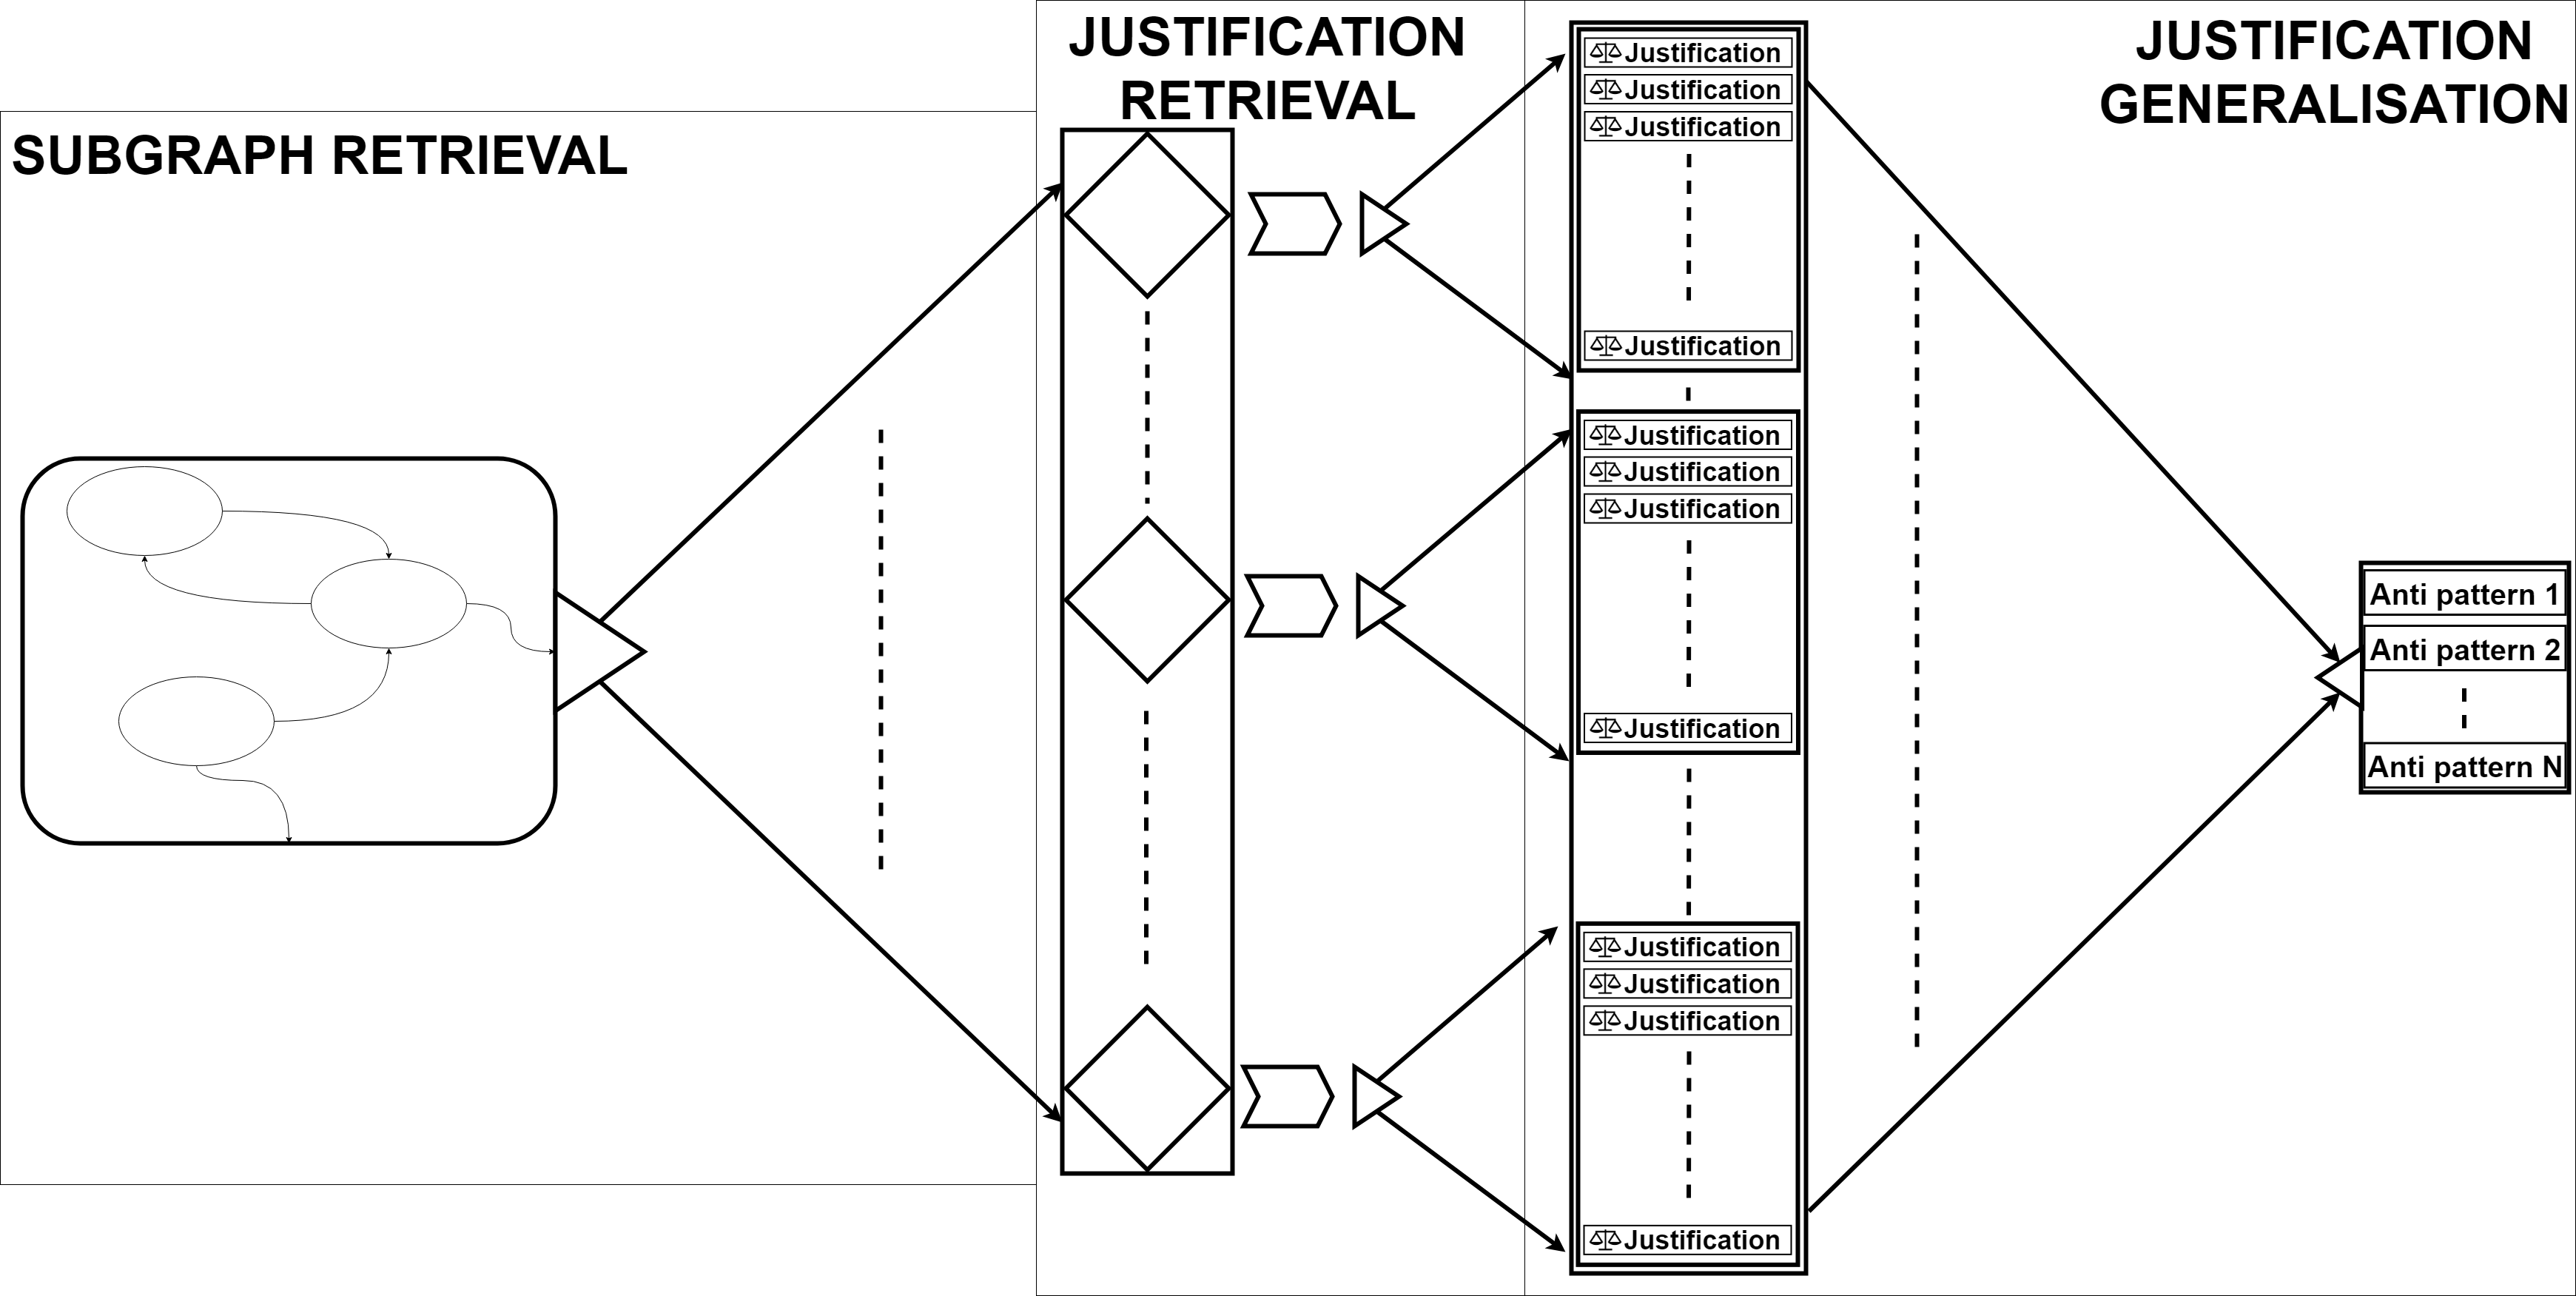
\includegraphics[width=\linewidth]{images/SimplifiedPipelineMissingPart.png}
		\caption{A schematic diagram that shows the pipeline used to extract subgraphs, find justifications and their `anti-patterns'.}
		\label{fig:simplePipeline}
	\end{figure}
	
	\section{Algorithmic overview and proof}
	We can prove that the algorithm can retrieve all `anti-patterns' from a given knowledge graph. We start by stating that it is possible to retrieve all inconsistency justifications in a knowledge graph, as has been proven by \cite{Horridge:2009}. Let us assume that we retrieved all justifications from a knowledge graph. We can know that also retrieved all `anti-patterns'. Each `anti-pattern' has one or more justifications that is contained in the knowledge graph. \\
	
	\begin{algorithm}
		\KwData{The knowledge graph that holds contradictions we want to extract}
		\KwResult{the set of `anti-patterns' found in the knowledge graph}
		
		retrieve all justifications in the knowledge graph\\
		\ForEach{justification in the list of justifications}{
			convert `anti-pattern' from justification\\
			\eIf{`anti-pattern' is not known}{
				add `anti-pattern' to list of known `anti-patterns'
			}{
				skip `anti-pattern' as we already know it.
			}
		}
		\Return list of `anti-patterns'\\
		\caption{Algorithmic view of the method}
	\end{algorithm}
	
	\section{Implementation of the Algorithm}
	Our extraction method consists of three aspects: Firstly, we retrieve smaller subgraphs from the knowledge graph from which. This phase is added as the size of a knowledge graph can be too large to check for inconsistencies in the complete graph. Secondly, from each subgraph, we check if the graph is inconsistent and retrieve the justifications. Finally, with the justifications, we create the `anti-patterns'. The entire pipeline is shown in figure \ref{fig:simplePipeline}.\\
	Our pipeline is designed to find `almost' all the `anti-patterns' in any knowledge graph. We implemented techniques to find these smaller inconsistent subgraphs with OWLAPI\cite{Horridge:2011} and Openllet\cite{Openllet:2019} which based on work of Pellet\cite{Pellet:2007}.\\
	
	\subsection{Subgraph retrieval}
	\begin{figure}
		\centering
		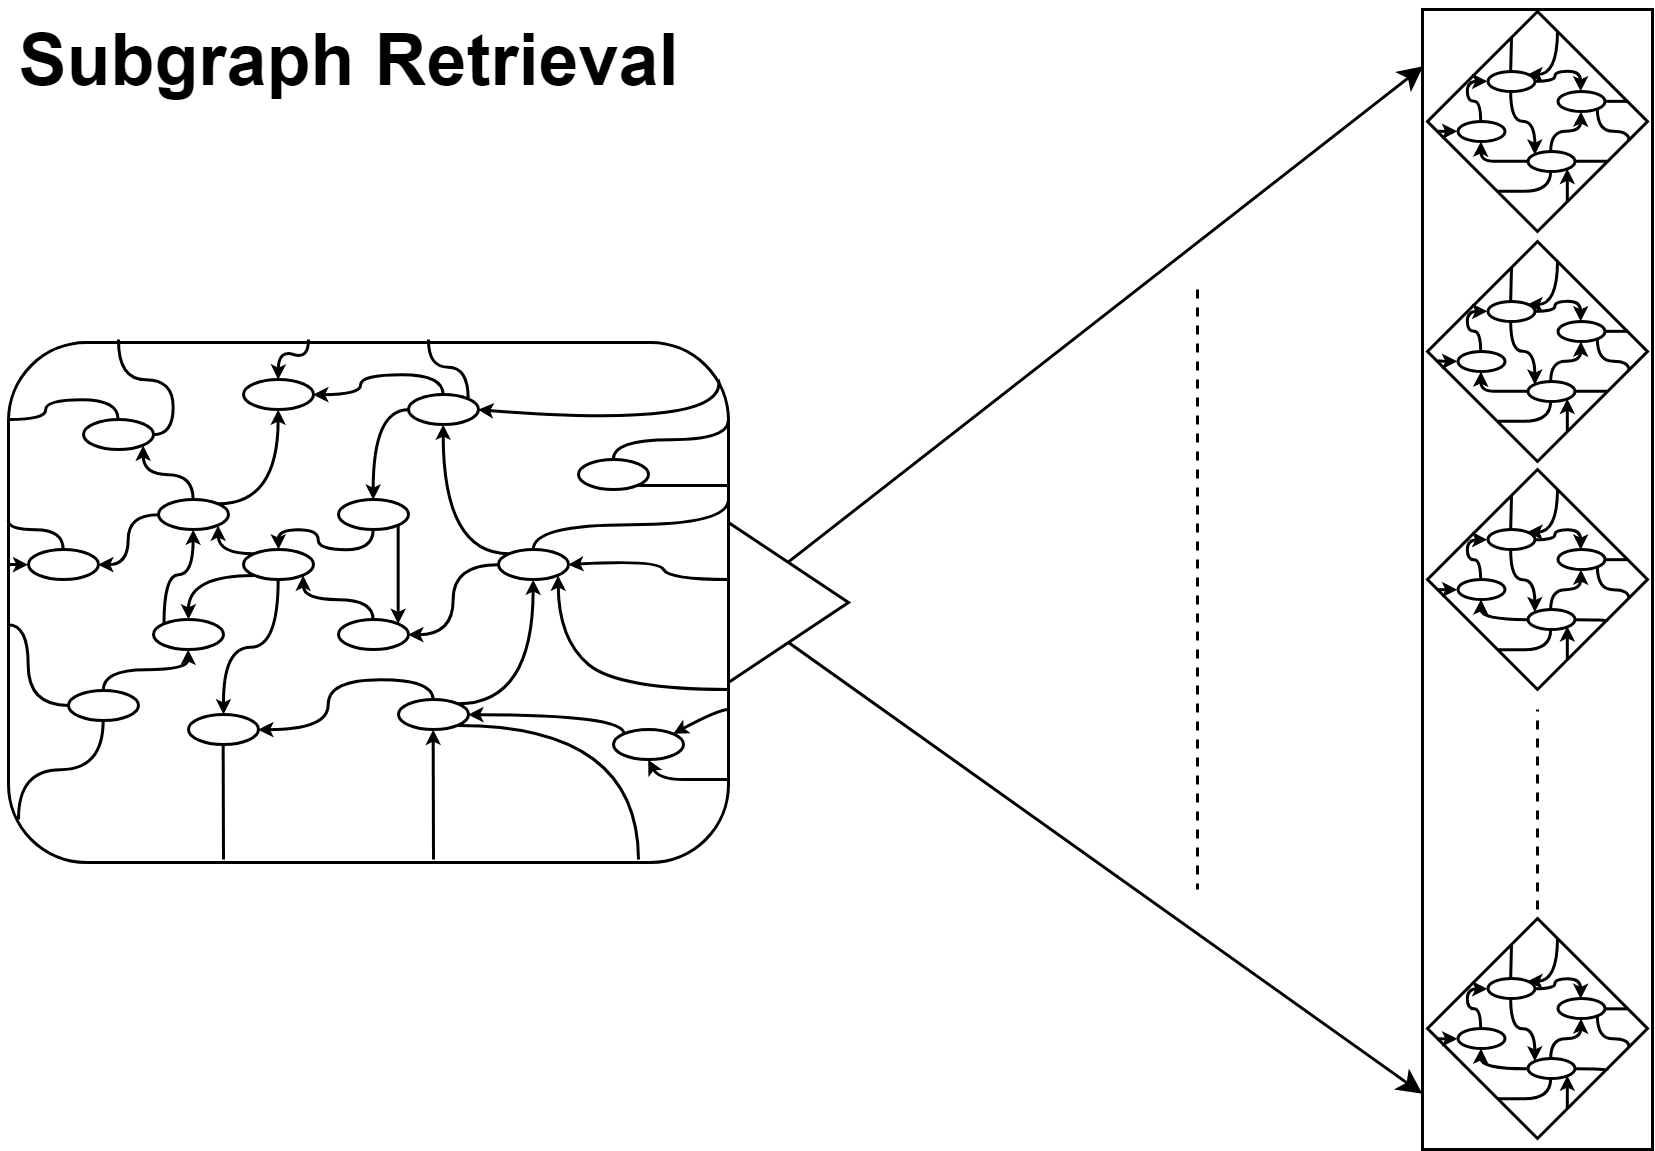
\includegraphics[width=\linewidth]{images/SubgraphRetrieval.png}
		\caption{A diagram that shows the retrieval and splitting of subgraphs from the knowledge graph.}
		\label{fig:subgraphRetrieval}
	\end{figure}
	\begin{figure}
		\centering
		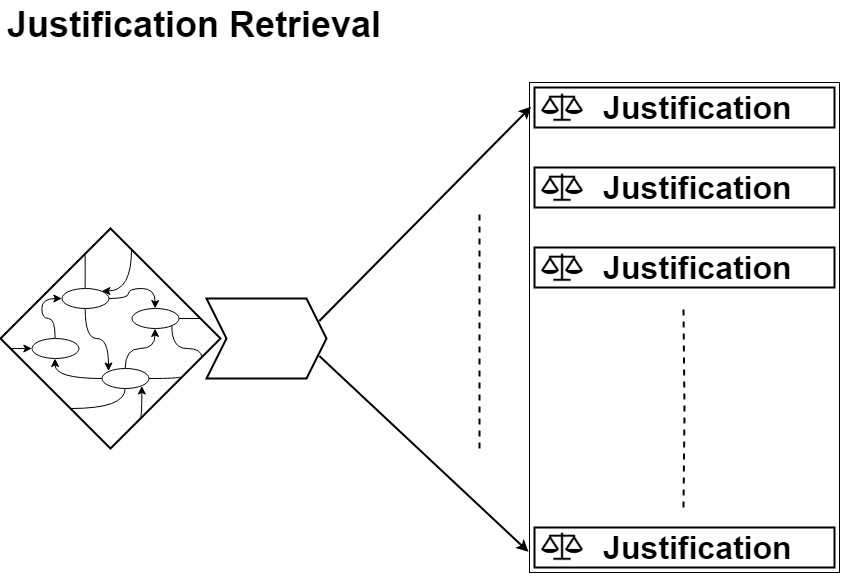
\includegraphics[width=\linewidth]{images/JustificationRetrieval.png}
		\caption{A diagram that shows the retrieval of justifications from a single subgraph.}
		\label{fig:JustificationRetrieval}
	\end{figure}
	
	Due to the large size of most knowledge graphs, running a justification retrieval algorithm over the complete knowledge graph, to retrieve all contradictions, would be impractical. To speed up this process, we decided to split the knowledge graph into smaller subgraphs to reduce the time the justification retrieval algorithm needs. Figure \ref{fig:subgraphRetrieval} shows the process of splitting the knowledge graph into smaller subgraphs.\\
	Each subgraph is generated by extending the root node. The root node is retrieved by taking a triple from the complete graph and taking the node that is in the subject position as the starting point. The graph is expanded by finding all the triples that have the root node as the subject, and we add these triples to the subgraph. If the amount of triples we added does not exceed the amount of triples we set as graph, we need to expand the graph further. To expand, all the nodes that were in the object position are now used as expansion nodes, so for each object, we find all the triples that match where the object is put in the subject position. We keep expanding the graph until it can not expand any further or the maximum amount of triples of 5000 triples is reached. The value of 5000 triples is chosen because it is large enough to hold almost all justification patterns but small enough that it does not take long to retrieve all justifications.\\
	This method to pick subgraphs from the knowledge graph does not guarantee completeness in terms of finding all the contradictions that can occur. In the experiments, we show that this method finds the `almost' all occurring contradictions. The reason for this is the redundancy we create by using subgraphs that overlap, without occurring too many time-consuming calculations. 
	
	\subsection{Justification retrieval}
	The knowledge graph is split into smaller subgraphs. We now move on the next step in the extraction pipeline, as shown in figure \ref{fig:JustificationRetrieval}.
	With the newly formed subgraphs, we start with the check if the graph is consistent or inconsistent. If the graph is consistent, we skip this graph, as the amount of contradictions is zero.\\ 
	If the graph is inconsistent, then we find the reason or reasons why. A graph can be inconsistent due to a single contradiction, or it can have multiple contradictions. 
	To find all the contradictions, we use the justifications algorithm in the Openllet reasoner. The justifications algorithm walks through the graph and finds the minimal justification for each contradiction. The algorithm continues to search for justifications until no more justification can be found in the graph. This is done for each subgraph, and all the justifications are then pushed through the extraction pipeline to the next stage.\\
	
	\subsection{Justification generalization to `anti-patterns'}
	While all justifications are different as each justification is a set of instantiated BTP, the underlying uninstantiated BGP does not have to be. The underlying BGP forms the basis of the `anti-patterns'. `Anti-patterns' describe a set of contradictions, that has been found in the inconsistent knowledge graph. The `anti-patterns' are generalized and can be used to locate inconsistencies in other knowledge graphs as well. In Figure \ref{fig:PatternGeneralizing}, we show the last part of the pipeline, the conversion of all justifications to a set of `anti-patterns'.
	
	\begin{figure}
		\centering
		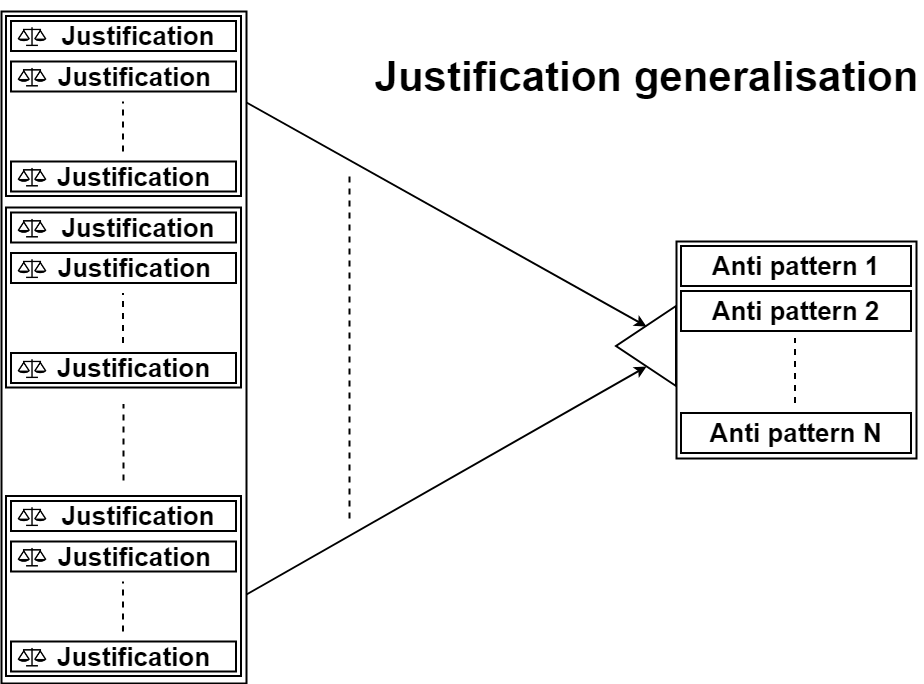
\includegraphics[width=\linewidth]{images/PatternGeneralizing.png}
		\caption{A schematic diagram showcasing how the justifications are transformed into Generalized inconsistency patterns.}
		\label{fig:PatternGeneralizing}
	\end{figure}
	\begin{figure}
		\centering
		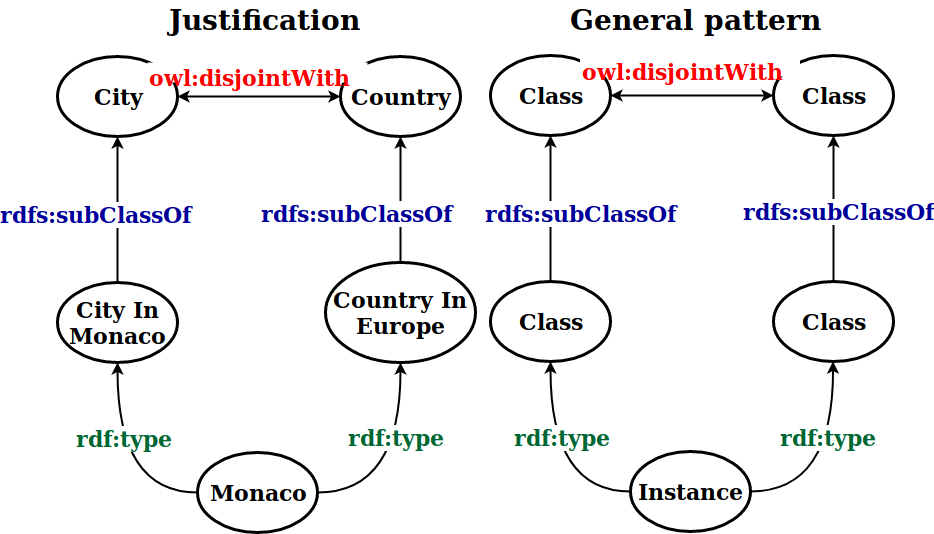
\includegraphics[width=\linewidth]{images/JustificationtoGeneral.png}
		\caption{A diagram that shows the transformation from Justification to a `anti-pattern'.}
		\label{fig:JustificationtoGeneral}
	\end{figure}
	
	
	To get the `anti-pattern' from the justification, we first generalise the justification by removing the instantiated subject and object on the nodes, as shown in figure \ref{fig:JustificationtoGeneral}. This gives the possibility to generalise the justification purely on its structure instead of its instantiated subject and object. While the information in the nodes is not essential, the information on the edges is. Graphs with different edges can be seen as different contradictions. \\
	If we, for example, change the `owl:disjointWith' into `rdfs:subclassOf' and transform one of the `rdfs:subclassOf' into an `owl:disjointWith' We have a different inconsistency pattern. For this reason, we need to store the edges in the `anti-pattern'.\\
	With the justifications now devoid of information on the nodes, we now group the justifications per `anti-pattern'. This means that each justification that has the same underlying `anti-pattern' is isomorphic, even with respect to the edges in the pattern. There some are exceptions to this rule, with for example `rdf:domain', and `rdf:range'.\\
	To find these isomorphisms, we have implemented a version of the VF2 algorithm\cite{LCordella:2004}, with the addition to the algorithm that we also match the edges of the two justifications. Checking if two graphs are isomorphic is NP-intermediate. Therefore we added in additional heuristics to filter the graphs first before we apply the VF2 algorithm. Firstly we check if a graph has the same number of vertices, the same number of edges, the same amount of degrees, and in our case it also needs to have the same amount of edges based on the edge types we have. If all the heuristics match then we apply the VF2 algorithm to the two justifications to find if they have the same `anti-pattern'. If the algorithm matches a justification to the found `anti-patterns', it adds this particular justification to this `anti-patterns', but if no pattern can be matched to the justification, a new `anti-patterns' is formed from this justification. This algorithm continues until all patterns have been matched to their correct `anti-pattern'.\\
	
	\section{Design decisions}
	To speed up the process for finding all `anti-patterns' in large knowledge graphs, we made design decisions that no longer guarantee that we can find all `anti-patterns'. We needed to implement these design decisions as it would else be intractable to locate all `anti-patterns'. 
	The first decision is to split the knowledge graph into smaller subgraphs. This makes it possible to for the reasoner to quickly check if the subgraph is consistent and retrieve all `anti-patterns' from the subgraph. To make sure we still find each `anti-pattern' we overlap the subgraphs such that it is improbable that we miss an contradiction because the contradiction was split and put into two different subgraphs.\\
	The second design decision is that we put in a cut off into the number of justifications the reasoner can find in the subgraph. We put this cut off in there deliberately. The reasoner, Openllet can continue indefinitely to find new justifications in a graph if no cut off is given \cite{Openllet:2019}. So this was one of the constraints that we needed to implement due to the chosen reasoner. 
	The final algorithm is shown in algorithm \ref{finalAlgorithm}.\\
	\\
	\begin{algorithm}
		\KwData{The knowledge graph that holds contradictions we want to extract}
		\KwResult{the set of `anti-patterns' found in the knowledge graph}
		KnowledgeSubgraphs split(knowledge graph)\\
		
		\ForEach{subgraph \textbf{in} KnowledgeSubgraphs }{
			retrieve contradictions in the subgraph, max 500.\\
			\ForEach{contradiction in list of contradictions}{
				convert `anti-pattern' from contradiction\\
				\eIf{`anti-pattern' is not known}{
					add `anti-pattern' to list of known `anti-patterns'
				}{
					skip `anti-pattern' as we already know it.
				}
			}
		}
		\Return list of `anti-patterns'\\
		\caption{Algorithmic view of the method}
		\label{finalAlgorithm}
	\end{algorithm}
	
	\newpage
	
	\chapter{Internal validation}\label{internalvalidation}
	
	\section{Data}
	We introduce the first two datasets that we use in this work, namely the Pizza-ontology and LOD-a-lot.
	
	\subsection{Pizza-ontology}
	The first ontology we use in our work is the pizza ontology. It is developed by Manchester university \cite{pizza}. The ontology describes pizza's and is used as an example ontology for prot\'{e}g\'{e} to explain how ontologies are created and how an ontology is used and expanded. The advantage of using this ontology over others, or own made, is that this ontology is widely known, everyone can find this ontology on the web. The ontology is a concrete example. We all know what a pizza is and what goes and does not go with a pizza. \\
	
	\subsection{LOD-a-lot}
	The second dataset we use is the LOD-a-lot\cite{JavierD:2017} knowledge graph. The LOD-a-lot is created by Javier David Fernandez Garcia, Wouter Beek, Miguel A. Martínez-Prieto and Mario Arias, and holds more than 28 billion statements, from a collection of 600 thousand datasets. The size of this dataset of 28 billion triples. The heterogeneous datasets that have been used to create this knowledge graph make it great for contradiction retrieval. As the number of different datasets could make it possible to find different sets of contradictions.
	
	\section{Experimental Setup}
	\textit{Method and Implementation software}. Both the method and the implementations, which we explain in section \ref{Method} and in section \ref{Implementation} have been written in JAVA. We choose JAVA as the programming language for the number of libraries that have been made available in JAVA. The most important libraries we used for the implementation are, Jena, rdf2hdt, openllet and OWLapi, all available as open source. It is noted that the retrieval of the `anti-patterns' has been done on the LOD server, as it took considerable resources and time to retrieve the `anti-patterns' from the LOD-a-lot. 
	
	\section{Experiment 1:  Can we design a pipeline that can retrieve a (sub-)set inconsistencies and translate the inconsistencies to `anti-patterns'?}
	% Describe how the creation of the inconsistencies from the lod cloud worked.
	\textit{Experiment description}. The purpose of this experiment is to show that we can indeed extract `anti-patterns' from an arbitrary knowledge graph. 
	To show that the pipeline works we have tested the algorithm on two extreme cases — the first case being the pizza ontology and the second case the LOD-a-lot.
	The pizza knowledge graph is great for measuring the completeness of the `anti-patterns' found. This shows it is measurable if the reasoner can find different inconsistencies. Which can be easily checked by hand.\\
	Because we can not prove that our pipeline guarantees the completeness, we test if the pipeline still retrieves all `anti-patterns' even when the size of the subgraph is smaller than the size of the knowledge graph.\\
	\textit{Analysis}. We compare the results of our method for retrieving the `anti-patterns' from the pizza ontology with the contradictions found by the reasoners in prot\'{e}g\'{e}, which we converted to `anti-patterns' by hand.
	The results are summarized in Table \ref{table:GraphStats}. The first column shows the size of triple subgraphs we used, In the first part of the algorithm we split the knowledge graph into smaller subgraphs, this size can be adjusted to improve speed vs redundant triples. In the table \ref{table:PizzaOntology} is shown that even with smaller subgraph sizes the algorithm still retrieves the same `anti-patterns' as the reasoners. The `anti-patterns' found by the reasoners are contradictions which are then transformed by hand to `anti-patterns'. 
	
	\begin{table}[!t]
		\begin{tabular}{|l|l|l|}
			\hline
			& Inconsistent? & Found inconsistencies \\ \hline \hline
			100 triple subgraphs     & Yes           & 2 \\ \hline
			500 triple subgraphs     & Yes           & 2 \\ \hline
			2,000 triple subgraphs     & Yes           & 2\\ \hline
			Pellet                     & Yes           & 2\\ \hline
			HermiT                     & Yes           & 2\\ \hline
		\end{tabular}
		\caption{table showing the reasoners to test the pizza ontology.}
		\label{table:PizzaOntology}
	\end{table}
	
	% Describe how the creation of the inconsistencies from the lod cloud worked.
	\section{Experiment 2: Anti-pattern Analysis} % Renaming
	% \section{Experiment 3: Anti-pattern Analysis} % Renaming
	\textit{Experiment description}. In experiment 1 we showed that it is possible to retrieve `anti-patterns' from a knowledge graph. In this experiment we analyze the `anti-patterns' we found in the LOD-a-lot. To get an overview for the `anti-patterns' that we found in the LOD-a-lot we designed a webpage. On this webpage we want to give several overviews over the `anti-patterns' found in the LOD-a-lot.
	
	\begin{figure}[!t]
		\subfloat[Circle-type `anti-pattern'.\label{fig:CircleAnti}]{%
			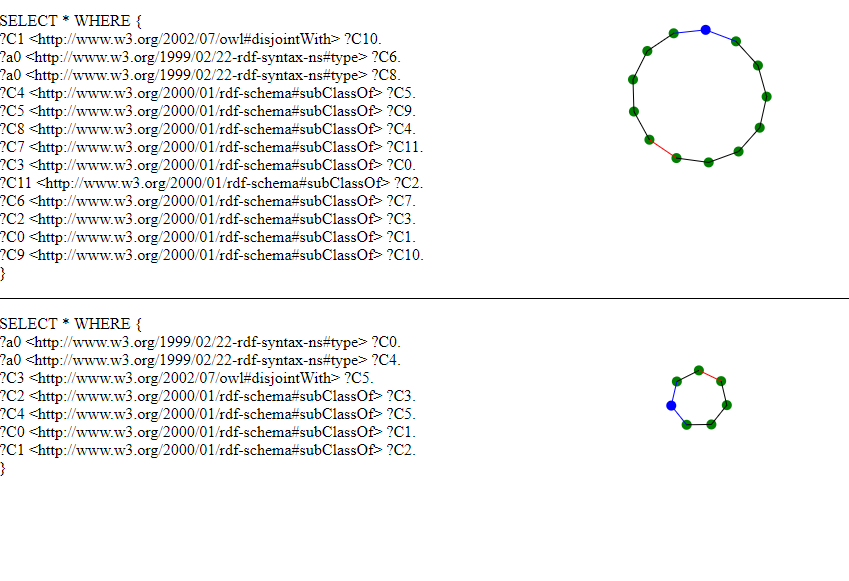
\includegraphics[width=0.5\textwidth]{images/Loop.png}
		}
		\subfloat[Kite-type `anti-pattern'.\label{fig:kiteAnti}]{%
			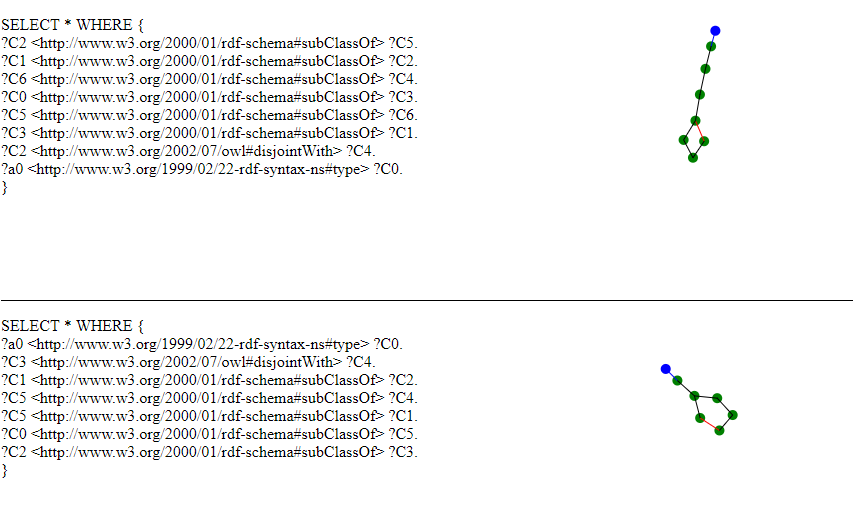
\includegraphics[width=0.5\textwidth]{images/Kite.png}
		}
	\end{figure}
	
	\textit{Analysis} In this experiment we created a webpage on\\ \url{https://thomasdegroot18.github.io/kbgenerator/Webpages/statisticsOverview.html} on which we compare the different `anti-patterns' we have found in the LOD-a-lot. On this webpage, we introduce the different types of contradictions we found. We show the `anti-patterns' via a visualization. We also give a formulation of the `anti-pattern'. And finally, we generate the SPARQL queries for every `anti-pattern'.  \\
	In the images \ref{fig:CircleAnti} and \ref{fig:kiteAnti} We show examples of the `anti-patterns' we found. We found that we can split the `anti-patterns' into four groups. The first group is are simple circles with with only two \textit{rdf:type}, \textit{rdfs:subClassOf} and \textit{owl:disjointWith}. These `anti-patterns' are the most common in a knowledge graph. The second group is a circle with an attachment. There is only one instance with \textit{rdf:type}. Then there are several \textit{rdfs:subClassOf} and one \textit{owl:disjointWith} relations. These groups are the second most common.  The third group is equal to the first group circle, but with the addition of different connections between the nodes that still make a contradiction but are less common, such as \textit{owl:equivalentWith} or \textit{rdfs:domain}. The fourth group is equal to the second group, but also with one or multiple other links such as \textit{owl:equivalentWith}. \\
	\newpage
	
	\chapter{Applications for `anti-patterns'}\label{Implementation}
	As shown in figure \ref{fig:PipelinePart45}, we designed two implementations that make use of `anti-patterns' that we found with the previous section. The first implementation is analysing the knowledge graph in its entirety. Looking at how the inconsistencies occur within the larger knowledge graph. We also use the analytics of the knowledge graph later in the sampling implementation. Secondly, we showcase that the sampling technique, with respect to the found `anti-patterns' in the graph that we used, produces similar, albeit smaller knowledge graphs.
	
	\section{Analysis tool kit for inconsistent knowledge graphs}
	In this paper, we show the implementation of analysing knowledge graphs on a set of characteristics. Our analysis of the knowledge graphs is split into two aspects. The first part is the retrieval of general statistics about the knowledge graph:
	\begin{itemize}
		\item The number of triples of the knowledge graph. An easy metric to calculate. This metric can be used as a basis for other more advanced metrics, such as ratio of size of the contradictions versus the size of the knowledge graph. This then can be used to compare the knowledge graphs.
		\item The number of distinct namespaces in the knowledge graph. This metric gives information about the amount of different `languages' e.g (OWL, RDFS, RDF, SKOS) that are used. 
		\item The distribution of indegree over all the nodes. Which are the counts of all the ingoing links. This can be seen as the amount of predicate-object links counted per object.
		\item The distribution of outdegree over all the nodes. Which are the counts of all the outgoing links. This can be seen as the amount of subject-predicate links counted per subject.
		\item The distribution of the Clustering Coefficient over all the nodes in the graph. This is the degree in which nodes cluster together. Which could be an indication of contradictions.  
	\end{itemize}
	The second part of the analysis is specifically aimed at inconsistency statistics. We locate all contradictions that match the `anti-patterns' that have been found by retrieving `almost' all `anti-patterns' from the LOD-a-lot. With the `anti-patterns' we can retrieve the needed statistics that characterise the knowledge graph. The metrics that are used in our analysis are:

	\begin{itemize}
		\item Amount of `anti-patterns' in the knowledge graph. This a count of the amount of different anti-patterns found in the knowledge graph. With more `anti-patterns' found meaning that there are more distinct contradictions been made in the data.
		\item Largest `anti-patterns' by a number of basic triple patterns found in the knowledge graph. Larger `anti-patterns' could indicate mistakes made by computers instead of humans.
		\item Distribution of the occurrences of contradictions found in the knowledge graph. The distribution of the `anti-patterns' is an ranked list. 
		\item Distribution of the sizes of `anti-patterns' found in the knowledge graph. The distribution is according to the size of the `anti-pattern'. Giving an overview if size of the `anti-pattern' can be related to the amount of occurences.
	\end{itemize} 
	\begin{figure}[!t]
	\subfloat[This diagram shows one of the usecases for the `anti-patterns', namely Analytics.\label{fig:AnalyticsDrawing}]{%
		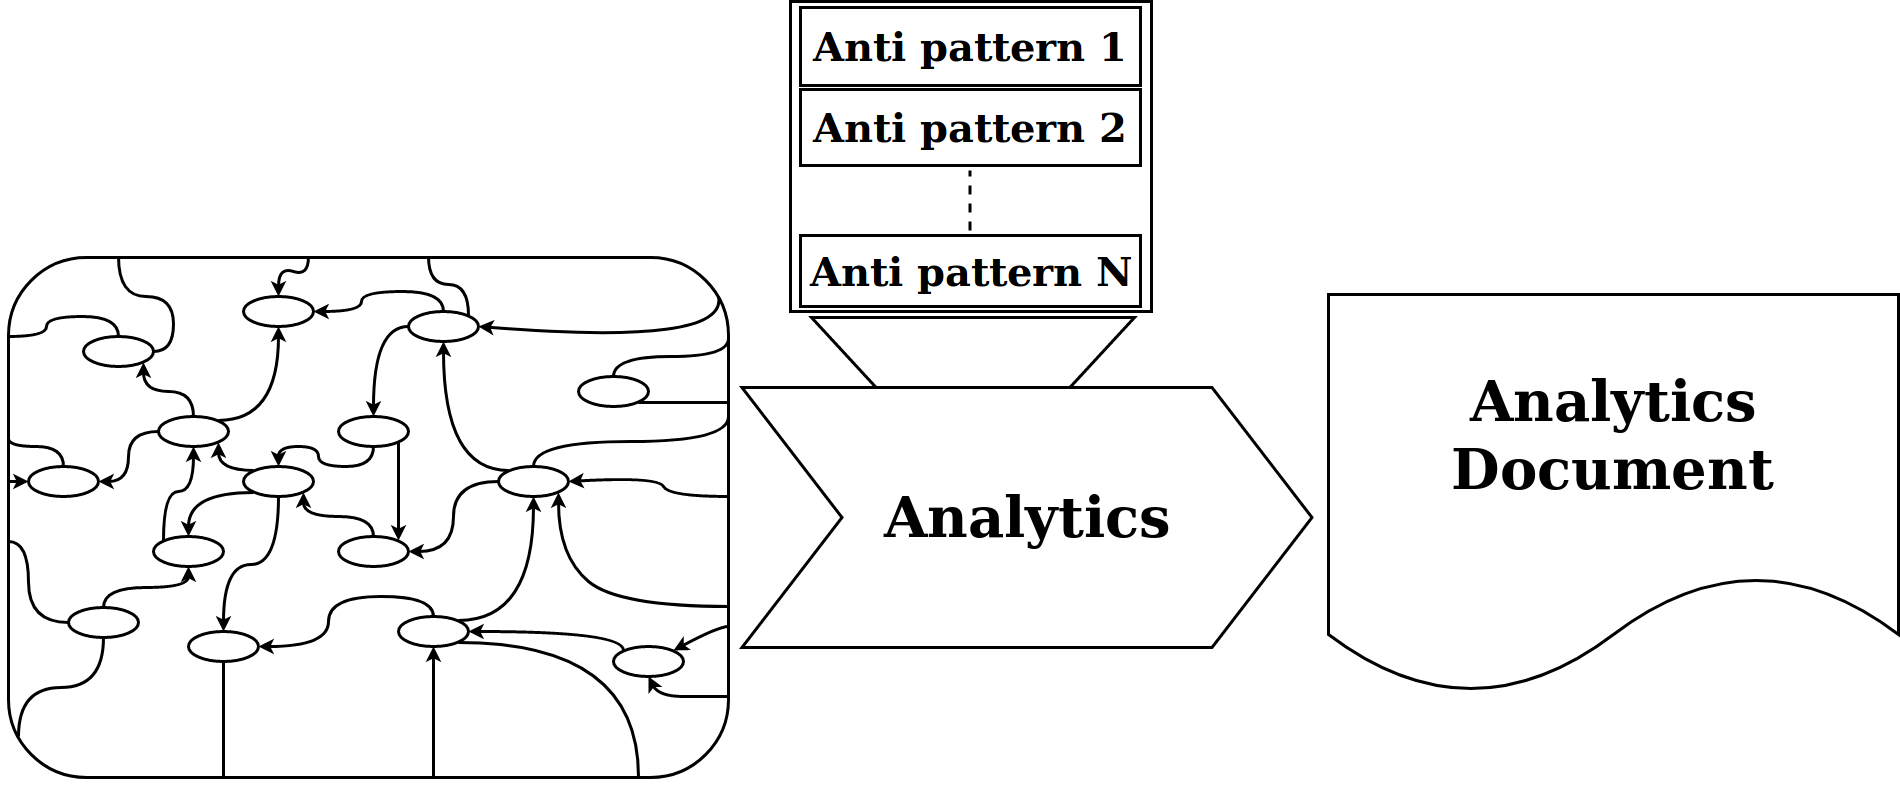
\includegraphics[width=0.45\textwidth]{images/AnalyticsDrawing.png}
	}
		\subfloat[This diagram shows the second usecase for the `anti-patterns', Sampling.\label{fig:SamplingDrawing}]{%
	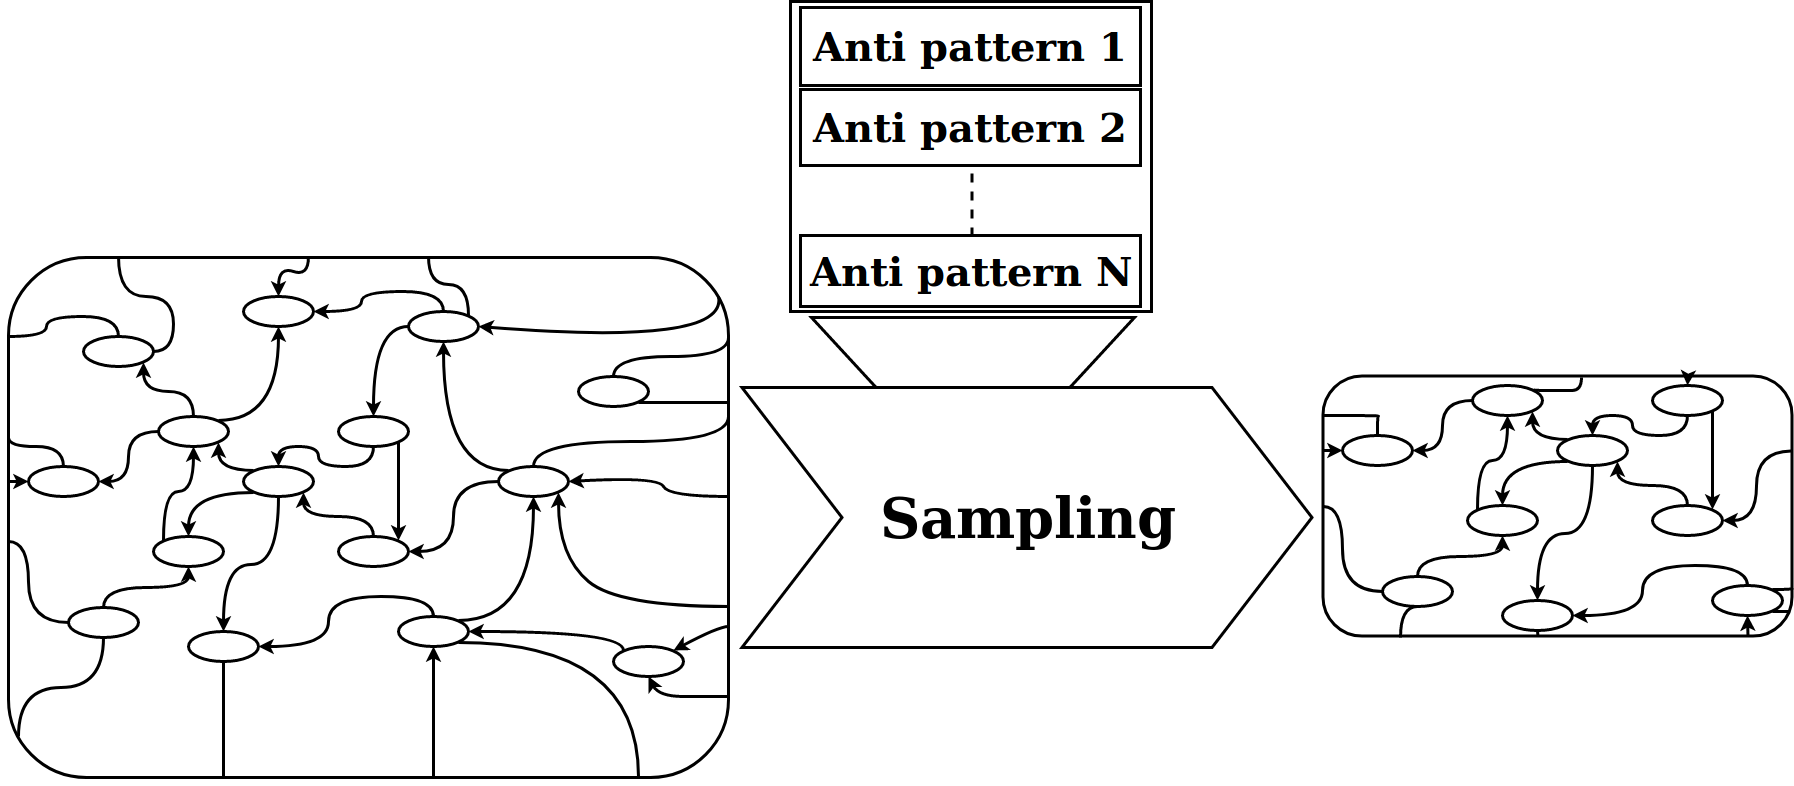
\includegraphics[width=0.45\textwidth]{images/SamplingDrawing.png}
}
	\caption{zoomed in diagram of the final parts of the pipelines.}
	\label{fig:PipelinePart45}
\end{figure}
	
	\section{Sampling toolkit for inconsistent knowledge graphs}
	The second implementation that makes use of the `anti-patterns' is the implementation of sampling a knowledge graph. In this paper, the goal of sampling is to sample a knowledge graph into a smaller partition with two constraints. The first constraint is that the knowledge graph stays connected. Secondly, we give the user the possibility to choose a set of `anti-patterns' and the minimal amount of contradictions that can be in the sample.
	Sampling inconsistent knowledge graphs is tricky, with the contraints we set for us. Most sampling techniques pick a random node as their starting point for sampling. For example the random walks, start on a random node and walk around and chain the links and other nodes to the starting node to generate a sample. This would make the graph always connected, but we can not add random contradictions into the graph without guaranteeing connections between the contradictions via the random walks. Due to this, we need to design our own sampling technique which can solve the problem we set with our constraints.
	Our algorithm instead uses random constrained deletion; this algorithm randomly deletes triples that can be safely deleted. There are triples that can not be deleted.\\
	The first set of triples that can not be deleted are the triples that describe the contradictions, see number 1 in figure \ref{fig:sampling}. To make sure that contradictions are not deleted, we start by building an HDT\cite{FMPGPA:13}\cite{MPAF:12} that stores all the triples that make up these contradictions. We use a SPARQL query to find the results of each of the `anti-patterns', and retrieve the number of contradictions the user wanted as BTPs. The triples are then combined and converted to an HDT. The algorithm can now check if a triple can be safely deleted. By checking if the triple is not present in the HDT.\\
	The second set of triples that can not be deleted are the triples that break the to sample graph into smaller subgraphs, see number 2 in figure \ref{fig:sampling}. To negate this problem the algorithm uses local connectedness. A triple may only be safely deleted if there is a second path that connects the object and the subject without having to pass through the severed link.
	\begin{figure}
	\centering
	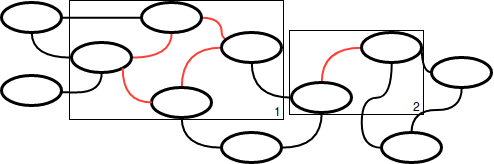
\includegraphics[width=\linewidth]{images/Sampling.png}
	\caption{figure shows types of undeletable triples, shown in red.}
	\label{fig:sampling}
\end{figure}
	There is one exception to the rule when either the subject or the object does not have any other links, the triple is then is also allowed to be deleted. With this, we can guarantee that the graph does not split into smaller subgraphs. 
	The sampling by random deletion now continues to delete triples until the sample reaches the size given by the user, or when it is no longer able to delete triples. This can happen either because the only triples that can be deleted split the graph into subgraphs, and/or the only triples that can be safely deleted belong to the non-deletable contradictions.
	
	\begin{algorithm}
	\KwData{knowledge graph we need to sample.}
	\KwResult{Sampled knowledge graph}
	retrieve all protected inconsistencies(KnowledgeGraph) \\
	\ForEach{triple \textbf{in} KnowledgeGraph }{
		\eIf{triple not belongs to protected inconsistency}{
			\eIf{triple has local connectedness}{
				remove triple
			}{
				skip triple.
			}
		}{
			skip triple.
		}
		
	}
	\Return Sampled knowledge graph\\
	\caption{Algorithmic view of the sampling method}
	\label{High top view}
\end{algorithm}
	
	\newpage
	\chapter{External validation}\label{externalvalidation}
	Next, we will show the results of the two implementations we designed, which we will also analyze. In these experiments, we use YAGO, and DBpedia, DBLP for analysis and sampling, as well as the `anti-patterns' from the LOD-a-lot as the `anti-pattern' input. With the expectation that the `anti-patterns' from the LOD-a-lot will encompass all the `anti-patterns' from the to sample datasets.\\
	
	\section{Data}
	In chapter \ref{internalvalidation} we introduced pizza and LOD-a-lot knowledge graphs. In this chapter, we introduce the final three datasets, namely DBpedia, DBLP and YAGO.
	
	\subsection{YAGO}
	The first dataset we will use for experimentation is YAGO\cite{YAGO2:2013}, this dataset has derived 160 million statements about 10 million entities, from Wikipedia, WordNet and GeoNames. This dataset is made open source and is a joint project of the Max Planck Institute for Informatics and the Telecom ParisTech University. The dataset has a temporal and spatial dimension, making it prone to contradictions. The dataset is also manually evaluated and is according to Hoffart et al\cite{YAGO2:2013} not a mistake-free dataset.
	
	\subsection{DBpedia}
	DBpedia\cite{DBpedia} is a crowdsourced project that extracts structural information from the Wikimedia, the foundation on which Wikipedia, but also others, such as Wikibooks, Wiktionary, and wiki data is based. DBpedia is an ongoing project, and at this moment their knowledge graph consists out of 1 billion statements about 4.58 million objects in the English version, and in total 9.5 billion statements if we combine all other languages as well. In this work, we focus on only the English version, as this has already been transformed into the correct file format for us. 
	
	\subsection{DBLP}
	dblp\cite{DBLP} The dblp knowledge graph is a large knowledge graph that stores bibliographic information on major computer science publications. It has grown from a small experimental knowledge graph to a popularly used knowledge graph that is used for testing and benchmarking. The knowledge graph contains 55 million triples.
	
	\subsection{Wordnet}
	Wordnet is a smaller knowledge graph containing a larger number of English nouns, verbs, adjectives and adverbs all grouped. The words have been linked, and can be used as thesaurus. The dataset consists out of 5.5 million triples for 118.000 words.
	
	\subsection{swdf}
	A small dataset comprising out of 242.000 triples. The dataset is small test case dataset that is mostly used by researchers to use as a testcase for algorithms. In this case we use the dataset as testcase for our analysis algorithm.
	
	\section{Experiment 3: Implementation 1, Analysing inconsistent graphs}
	%\section{Experiment 4: Implementation 1, Analysing inconsistent graphs}
	\textit{Experiment description}. We are retrieving the statistics from several knowledge graphs differing in size. In this experiment, we retrieve relevant statistics from YAGO, DBpedia. The two inconsistent knowledge graphs. And we use three smaller consistent knowledge graphs, wordnet31, dblp-2012-11-28b, swdf as control knowledge graphs. The statistics we retrieve are explained in chapter \ref{Implementation}.  \\
	
	\textit{Analysis}. Table \ref{table:GraphStats} shows the analytics about the knowledge graphs we retrieved from our analytics toolkit. As noticed, the results show several distinctions between the three different knowledge graphs. Most important differences are the size and the number of different namespaces. The important statistics are the largest `anti-pattern', that can be found in the data. Finally the amount of distinct `anti-patterns' that can be found in the knowledge graph. Here we can see that size does matter in the amount of different `anti-patterns' found, but is most noticeable with smaller graphs. \\
	Figures \ref{fig:indegree},  \ref{fig:outdegree},  \ref{fig:Coeff}, show the different distribution of statistics of the knowledge graphs. We can distinctly see different knowledge graphs in the data. The first thing to notice is the drop in the graphs in \ref{fig:indegree}. In all but the swdf knowledge graph, we can see a visible drop in the number of ingoing connections, between 10 and 100 incoming connections. \\
	The outgoing connections in graph \ref{fig:outdegree} do not have interesting characteristics but will be useful for comparing the sampling method in the next experiment. 
	The final graph about the knowledge graph statistics \ref{fig:Coeff} shows the clustering coefficient most important to note is the high amplitude graph for dblp-2012-11-28b. \\
\begin{table}[!t]
	\centering
	\resizebox{\textwidth}{!}{
		\begin{tabular}{l|llll}
			\hline
			& Size          & Namespaces  & Amount of `Anti-patterns' &  Largest Inconsistency \\ \hline \hline
			LOD & 28,362,198,927 & - & 222 & 19\\
			DBpedia & 1,040,358,853            & 20                            & 13                         & 12                        \\
			YAGO     & 158,991,568             & 11                            & 135                        & 16                        \\
			DBLP & 55,586,971 	   & 7  & 0 & 0\\
			wordnet  & 5,558,748                & 5                                 & 0 & 0\\
			swdf         & 242,256                & 22 & 0 & 0\\
			
	\end{tabular}}
	\caption{table showing several statistics about graphs.}
	\label{table:GraphStats}
\end{table}

\begin{figure}[!t]
	\subfloat[The distribution of indegree over all nodes.\label{fig:indegree}]{%
		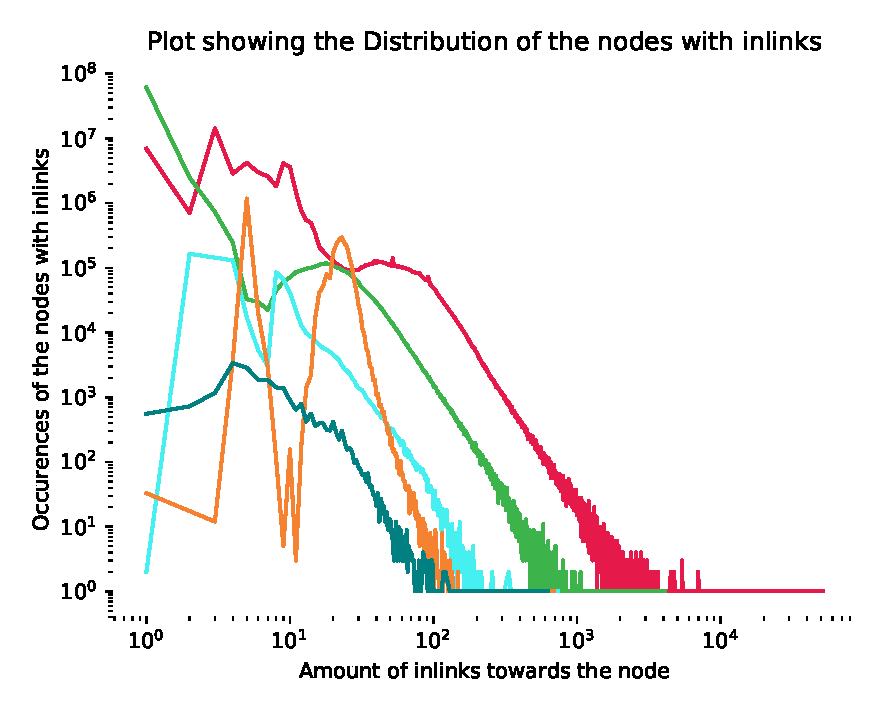
\includegraphics[width=0.33\textwidth]{images/figure4.eps}
	}
	\subfloat[The distribution of outdegree over all nodes.\label{fig:outdegree}]{%
		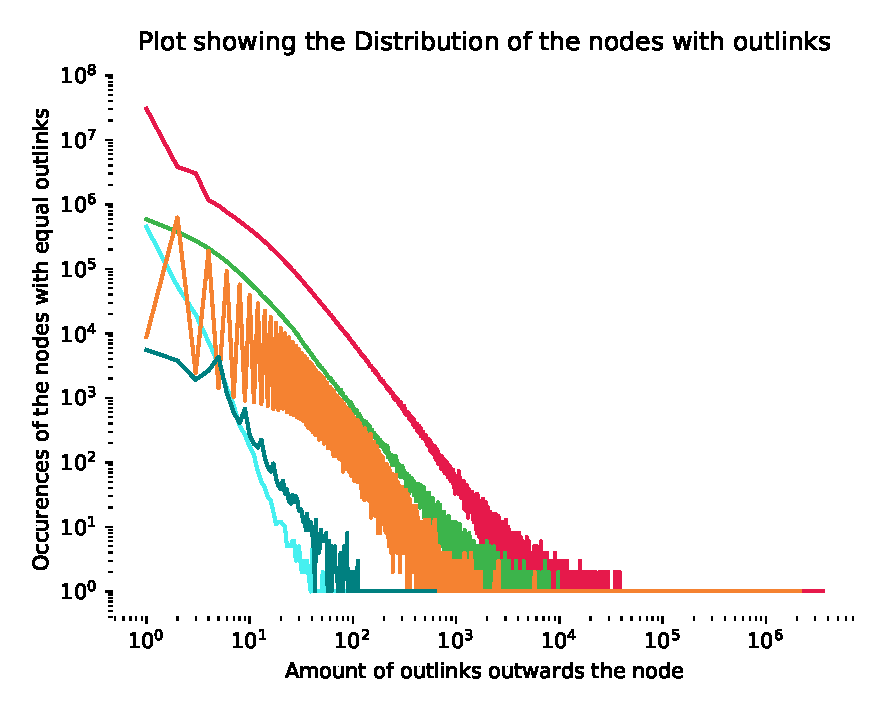
\includegraphics[width=0.33\textwidth]{images/figure5.eps}
	}
	\subfloat[The distribution of the Clustering Coefficient over all nodes.\label{fig:Coeff}]{%
		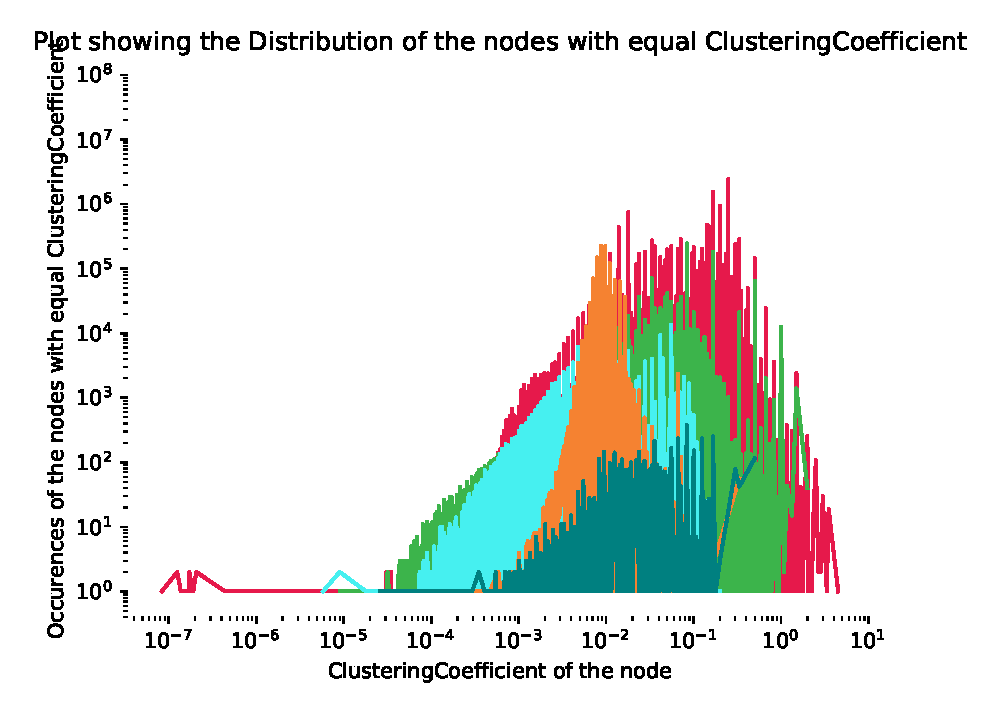
\includegraphics[width=0.33\textwidth]{images/figure6.eps}
	}
\end{figure}

	
	The final two graphs show the curves for the two inconsistent knowledge graphs. DBpedia and YAGO. Both have `anti-patterns' meaning that the knowledge graphs are inconsistent. While the size of the knowledge graphs is different. The curve for both YAGO and DBpedia are similar. 
	
	
\begin{figure}[ht]
	\centering
	\subfloat[Plot showing the Distribution of size.\label{fig:DistributionSize}]{%
		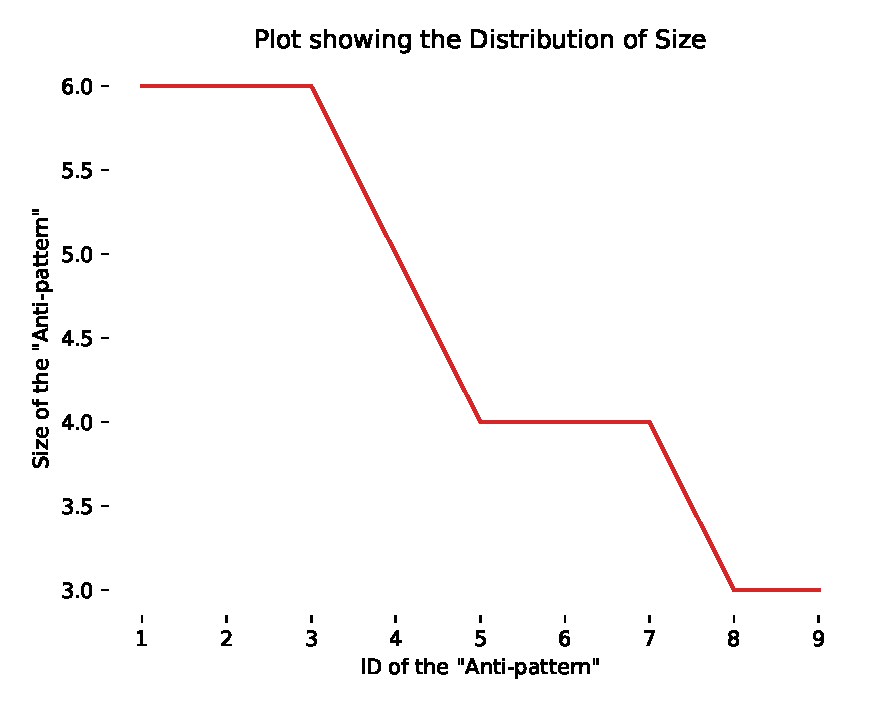
\includegraphics[width=0.33\textwidth]{images/figure1.eps}
	}
	\subfloat[Plot showing the Distribution of Distinct `anti-patterns'.\label{fig:SizeDistinct}]{%
		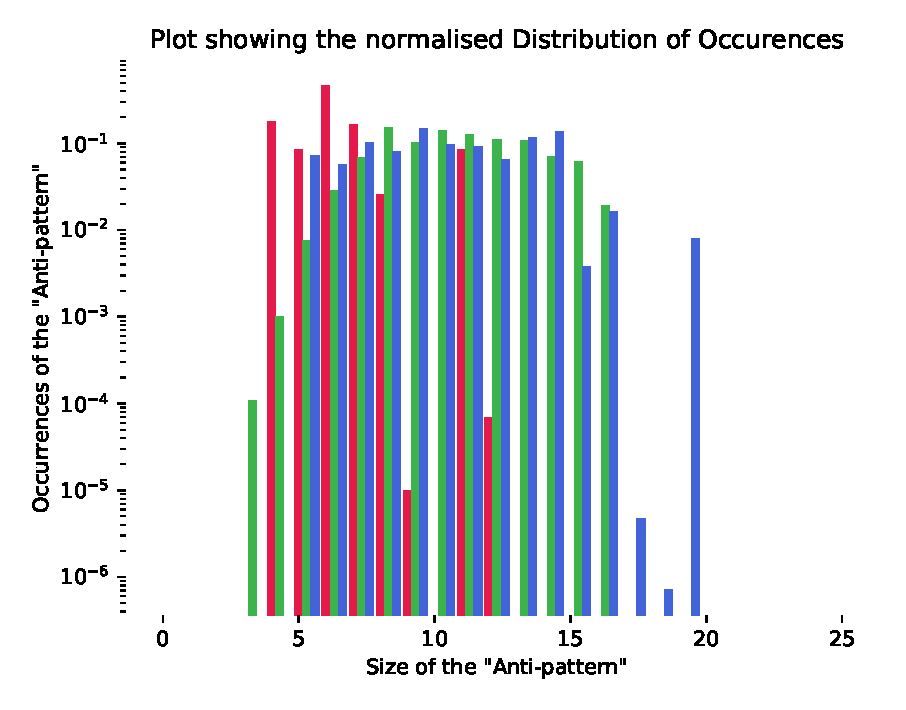
\includegraphics[width=0.33\textwidth]{images/figure2.eps}
	}
	\subfloat[Plot showing the Distribution of occurrences.\label{fig:Distributionoccurrences}]{%
		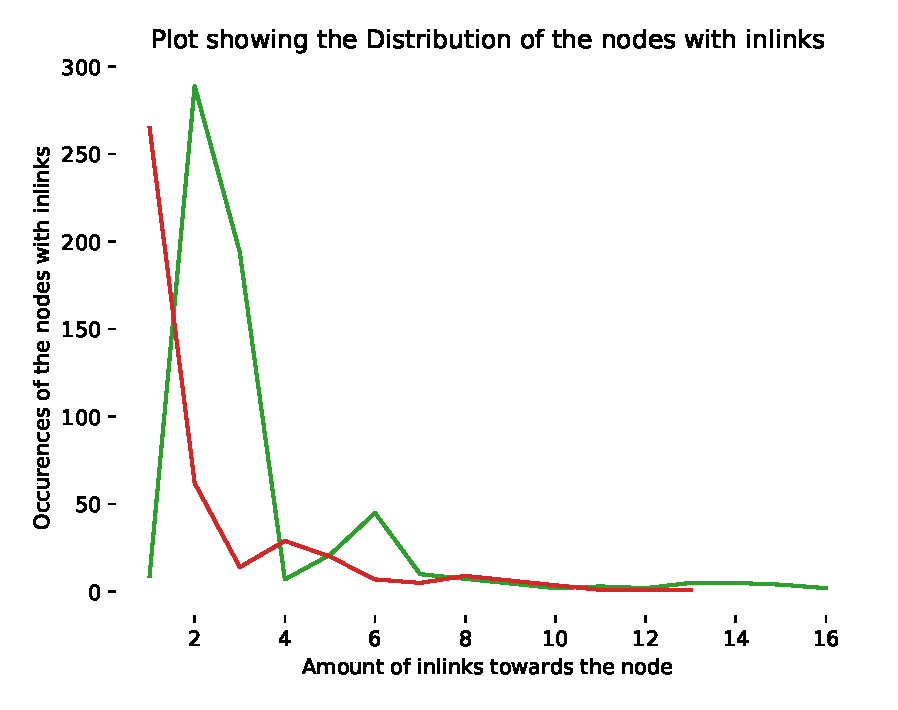
\includegraphics[width=0.33\textwidth]{images/figure3.eps}
	}
	\caption{Figures showing several statistics about the Anti patterns.}
	\label{fig:AntipatternStats}
\end{figure}

	% \section{Experiment 5: Use case 2, Sampling inconsistent graphs} 
	\section{Experiment 4: Use case 2, Sampling inconsistent graphs} 
	\textit{Experiment description}. To test sampling, a sample size of 20\% is taken. The paper by Jure Leskovec and Christos Faloutsos \cite{Leskovec:2006} shows that samples up to 15\% still hold the characteristics of the original graph well, even with simpler sampling methods. Choosing 20\% of the original knowledge graph, we make sure that the sampling is not having large effects on the characteristics of the sampled graph. We can, therefore, better compare the sampled knowledge graph with the original knowledge graph. \\
	
	
\begin{table}[!t]
	\centering
	\resizebox{\textwidth}{!}{
		\begin{tabular}{l|llllll}
			\hline
			& Size          & Namespaces  & Amount of `Anti-patterns' &  Largest Inconsistency \\ \hline \hline
			DBpedia-20\% & 83,464,390            & 2                            & 11                         & 12                        \\
			YAGO-20\%     & 62,562,330           & 7                             & 123                        & 16                        \\
			dblp-20\%  & 16,812,580 	& 3 							& 0 & 0
	\end{tabular}}
	\caption{table showing several statistics about graphs.}
	\label{table:GraphStatsSample}
\end{table}
	
	\textit{Analysis}. Table \ref{table:GraphStats} shows the analytics about the knowledge graph before the sampling. As noticed, the results show several distinctions between the three different knowledge graphs. Even though their expressiveness and the size do roughly match their number of namespaces and distinct predicates differ between the three test cases.\\
	Table \ref{table:GraphStatsSample} shows the analytics of the knowledge graphs after the sampling has been applied. The sample size is roughly one-fifth of the original size. The statistics of the sampled knowledge graph still match the original knowledge graph.
	Figures \ref{fig:indegree},  \ref{fig:outdegree},  \ref{fig:Coeff}, show the distribution of statistics of the knowledge graph. All graphs show different curves, but the most noticeable is the dip in the dblp line for the in degrees. 
	Figures \ref{fig:indegreeSample},  \ref{fig:outdegreeSample},  \ref{fig:CoeffSample} show the distribution of the statistics sampled knowledge graph. As noted, we can see that the distribution of the statistics does match the original knowledge graph. We can distinguish the graphs and match them to the original graphs. 
	In figure \ref{fig:indegreeSample} the sign of this is the obvious dip in the dblp line for the in degrees. Which, while smoothed is still characteristic of the dblp-2012-11-28b dataset. The same dips are also seen in the DBpedia sample and the YAGO sample.\\
	In figure \ref{fig:outdegreeSample} the same effects are visible. While the dblp has been smoothed out, which can be the effect of the sampling. All three lines follow the same angle as their original graphs.\\
	In figure \ref{fig:CoeffSample} it is visible that all three sampled knowledge graphs have the same shape in the clustering coefficient as their original knowledge graphs. While the respective sizes of the knowledge graphs make the plot harder to read, it can still be seen that the plots match the shapes of the original dataset.
	
\begin{figure}[!t]
	\subfloat[The distribution of indegree over all nodes of the sample.\label{fig:indegreeSample}]{%
		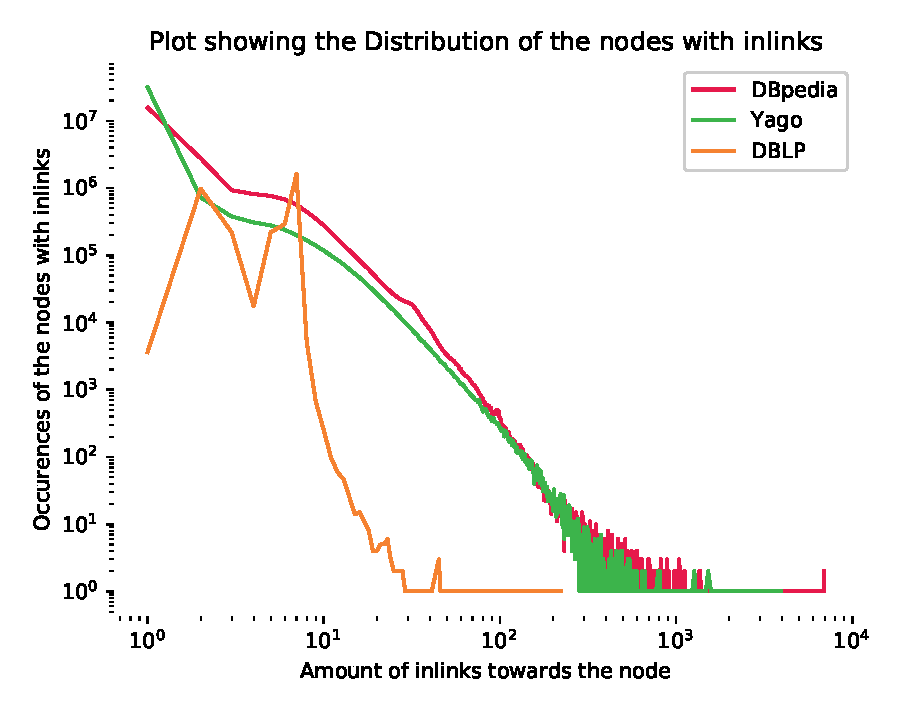
\includegraphics[width=0.33\textwidth]{images/Samplefigure4.eps}
	}
	\subfloat[The distribution of outdegree over all nodes of the sample.\label{fig:outdegreeSample}]{%
		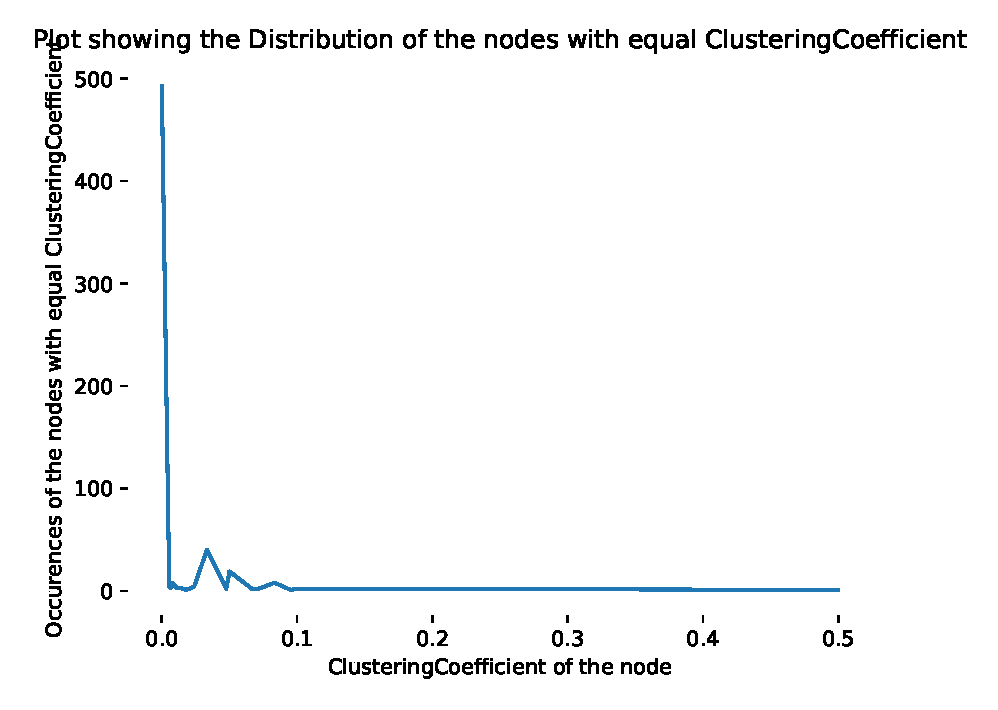
\includegraphics[width=0.33\textwidth]{images/Samplefigure5.eps}
	}
	\subfloat[The distribution of the Clustering Coefficient over all nodes of the sample.\label{fig:CoeffSample}]{%
		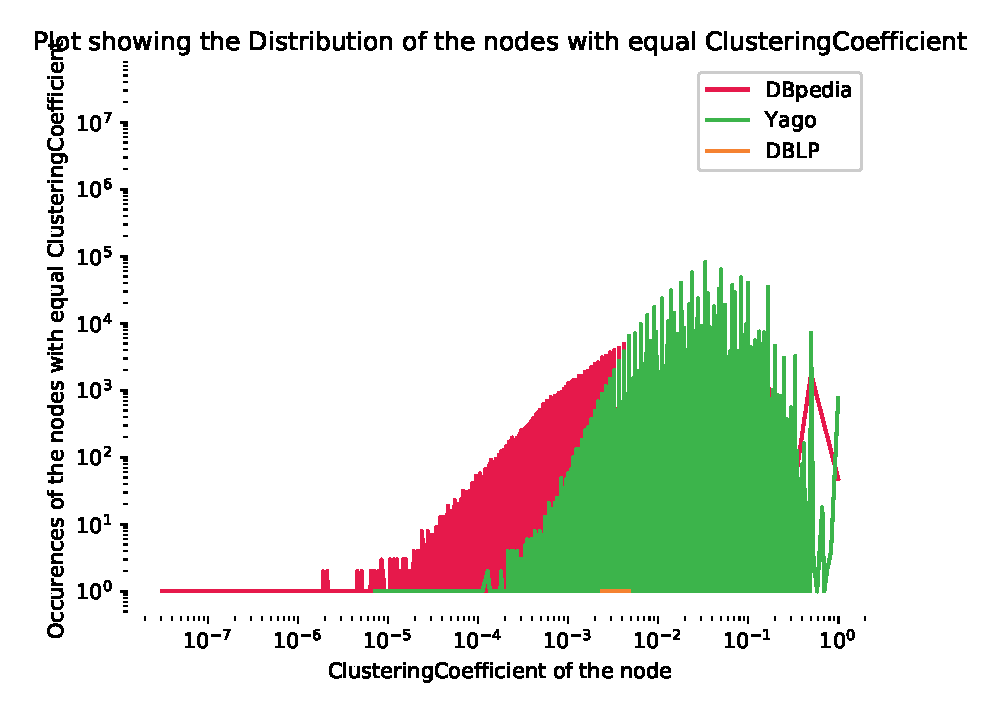
\includegraphics[width=0.33\textwidth]{images/Samplefigure6.eps}
	}
	\caption{Figures showing several statistics about graphs.}
	\label{fig:GraphStats}
\end{figure}
	
	
	Figure \ref{fig:SizeDistinctSample},\ref{fig:DistributionoccurrencesSample} and \ref{fig:DistributionSizeSample} show the distinct occurrences, distribution of occurrences and distinct `anti-patterns' per amount of triples for both the sample and original Knowledge Graph for Yago and DBpedia. They show very nicely that the sample have very similar properties w.r.t. inconsistencies to their larger originals, which was the main goal set of sampling. 
	
\begin{figure}[ht]
	\centering
	\subfloat[Plot showing the Distribution of `anti-pattern' size, for the sampled and original graph.\label{fig:DistributionSizeSample}]{%
		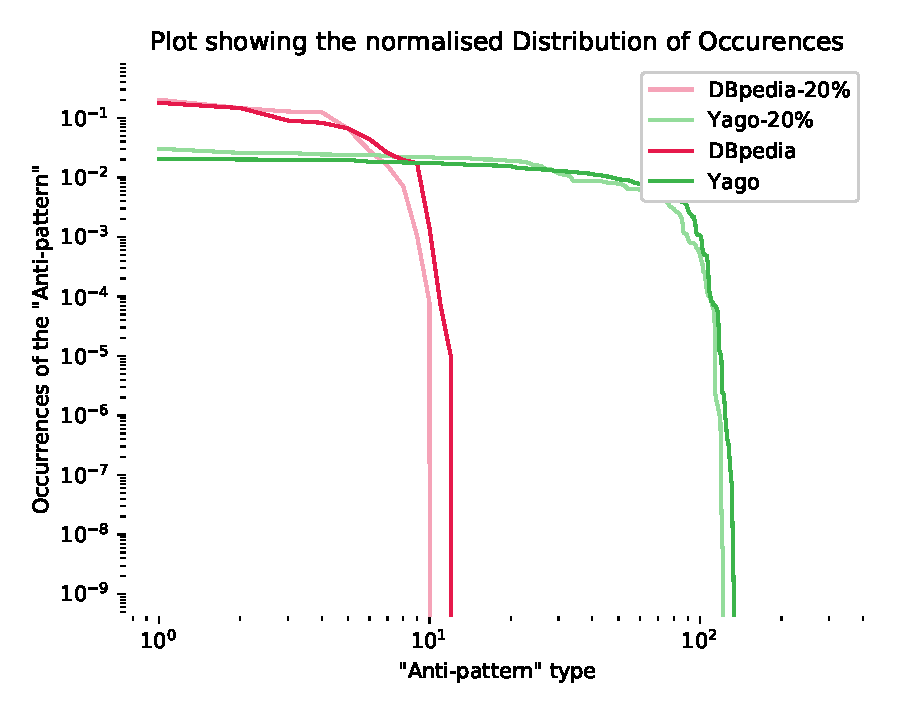
\includegraphics[width=0.33\textwidth]{images/Samplefigure1.eps}
	}
	\subfloat[Shows the distribution of distinct `anti-patterns', for the sampled and original graphs.\label{fig:SizeDistinctSample}]{%
		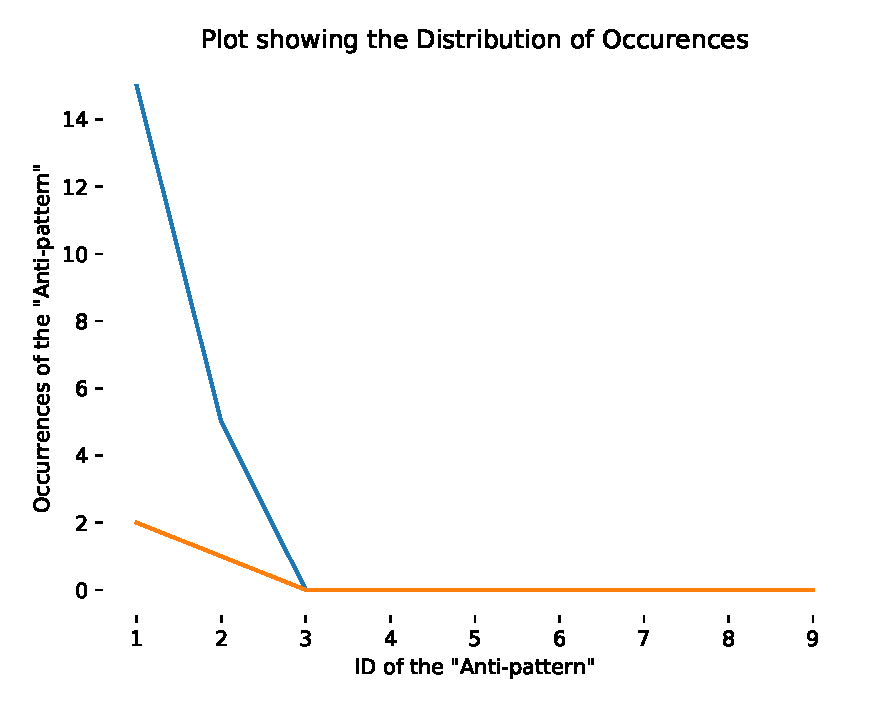
\includegraphics[width=0.33\textwidth]{images/Samplefigure2.eps}
	}
	\subfloat[Shows the distribution of occurrences, for the sampled and original graphs.\label{fig:DistributionoccurrencesSample}]{%
		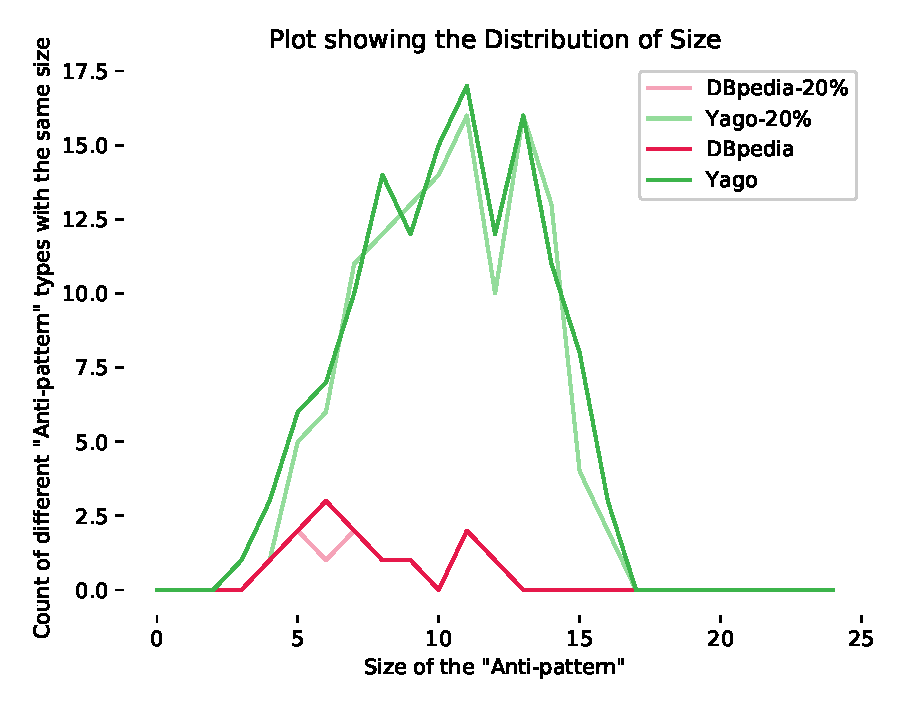
\includegraphics[width=0.33\textwidth]{images/Samplefigure3.eps}
	}
	\caption{Figures showing several statistics about the Anti patterns within the samples.}
	\label{fig:AntipatternStatsSample}
\end{figure}
	
	\newpage
	
	\chapter{Conclusion}\label{Conclusion}
	In this work, we describe an anti-pattern as a minimal set of uninstantiated basic triple patterns that match an inconsistent subgraph in a knowledge graph. The advantage of converting justifications of contradictions in `anti-patterns' is that now we can use `anti-patterns' to locate contradictions in other knowledge graphs, which is a good method with the generalization to `anti-patterns'. Transferring knowledge about contradictions from one graph to the next was not easy with only justifications, but the `anti-patterns' solve this problem. 
	Secondly, the generalisation saves the information space, as several justifications can be mapped onto a single `anti-pattern', and retrieving the justification from the knowledge graph can now be done using a simple query. Now using the `anti-patterns' finding how inconsistent a knowledge graph is can be asked by using just SPARQL. Although we can not prove that being devoid of `anti-patterns' will mean that the knowledge graph is consistent, at least we can say for sure that if there is an `anti-pattern' match, the knowledge graph is inconsistent, and how.  \\
	
	The second contribution we introduce in this work is the extraction pipeline. The pipeline has been designed to extract `anti-patterns' from any natural knowledge graph. In this work, we show that we can extract all `anti-patterns' from the knowledge graphs in our experiments. However, we can not prove that our implemented method will extract all `anti-patterns', due to the design decisions made in chapter \ref{Method}.\\ 
	
	The final contribution in this work are the two implementations, knowledge graph analysis and knowledge graph sampling with respect to `anti-patterns'. For knowledge graph analysis, we can now give qualitative and quantitative information about a knowledge graph concerning its inconsistency. In our experiments, we show relevant statistics that can be found using the `anti-patterns'. Using the analysis tool everybody can now check their knowledge graph for relevant statistics about their knowledge graph. \\
	
	Finally, for knowledge graph sampling, we showed that knowledge graph sampling with respect to `anti-pattern' is possible. We demonstrated this by sampling knowledge graphs by random deletion. We showed that sampled knowledge graphs still have the same characteristics with original knowledge graphs.\\
	
	We made both the toolkit, the extraction pipeline, as well as the tools for sampling and analysis available on Github. \\ \url{https://thomasdegroot18.github.io/kbgenerator/Webpages/statisticsOverview.html}. We also provide a range of `anti-patterns' with their equivalent SPARQL queries.\\
	\textit{Future Work}. We observed that `anti-patterns' follow the same distribution in each of the large knowledge graphs. the analysis of the `anti-patterns' also showed that most `anti-patterns' consist out of `rdfs:subclassOf' and `owl:disjointWith'. `rdfs:range' and `rdfs:domain' do not occur so often in the `anti-patterns'.
	We want to evaluate why `rdfs:range' and `rdfs:domain' do not occur so often in the `anti-patterns' and we would improve the generalisation of `anti-patterns', by creating more general types for `anti-patterns'. At the moment, we have only looked at the most common knowledge graphs. We would also like to investigate the lesser-known knowledge graphs, such that we can expand our knowledge about the `anti-patterns' that occur in less known ontologies or graphs. Which can give us more insights into all types of ontologies.\\
	
	Returning to Blaise Pascal, while we can not prove that our `anti-patterns' give the answers to consistent knowledge graphs, and the lack of `anti-patterns' will mean that a knowledge graph is devoid of mistakes. `Anti-patterns' will help us understand how contradictions in a knowledge graph come to be, and we use them to make the knowledge graphs cleaner.
	
	\newpage
	\bibliographystyle{plain}
	\bibliography{ThesisBib}
	
	
\end{document}